%%%%%%%%%%%%%%%%%%%%%%%%%%%%%%%%%%%%%%%%%%%%%%%%%%%%%%%%%%%%%%%%%%%%%
% LaTeX Template: Project Titlepage Modified (v 0.1) by rcx
%% Original Source: http://www.howtotex.com

\documentclass[12pt]{report}
\usepackage[a4paper]{geometry}
\usepackage[myheadings]{fullpage}
\usepackage{fancyhdr}
\usepackage{lastpage}
\usepackage{graphicx, wrapfig, subcaption, setspace, booktabs}
\usepackage[T1]{fontenc}
\usepackage[font=small, labelfont=bf]{caption}
\usepackage{fourier}
\usepackage[protrusion=true, expansion=true]{microtype}
\usepackage[english]{babel}
\usepackage{sectsty}
\usepackage{url, lipsum}
\usepackage{hyperref}
\usepackage{float}
\usepackage{mathptmx}
\usepackage{amsmath}
\usepackage{amssymb}
\usepackage{float}

\newcommand{\HRule}[1]{\rule{\linewidth}{#1}}
\onehalfspacing
\setcounter{tocdepth}{5}
\setcounter{secnumdepth}{5}

%-------------------------------------------------------------------------------
% HEADER & FOOTER
%-------------------------------------------------------------------------------
\pagestyle{fancy}
\fancyhf{}
\setlength\headheight{15pt}
\fancyhead[L]{Manual Version 1.0}
\fancyhead[R]{Multigenomic Entropy-Based Score (MEBS)}
\fancyfoot[R]{Page \thepage\ of \pageref{LastPage}}
%-------------------------------------------------------------------------------
% TITLE PAGE
%-------------------------------------------------------------------------------

\begin{document}

\title{ \normalsize \textsc{User's guide version 1.0}
		\\ [2.0cm]
		\HRule{0.5pt} \\
		\LARGE \textbf{\uppercase{MEBS}}\\
  \textbf{\uppercase{Multigenomic Entropy-Based Score}}      
		\HRule{2pt} \\ [0.5cm]
		\normalsize \today \vspace*{5\baselineskip}}

\date{}

\author{
		Valerie De Anda Torres (valdeanda@ciencias.unam.mx) \\ 
    Augusto Cesar Poot-Hernandez (augusto.poot@iimas.unam.mx) \\
		Bruno Contreras Moreira (bcontreras@eead.csic.es) }

\maketitle
\tableofcontents
\newpage

%-------------------------------------------------------------------------------
% Section title formatting
\sectionfont{\scshape}
\section{Installing}
The MEBS software is available as an open source package on the
\href{https://github.com/eead-csic-compbio/metagenome_Pfam_score}{GitHub}
repository.

First cloning the repository via the following commands

\begin{verbatim}
git clone https://github.com/eead-csic-compbio/metagenome_Pfam_score
\end{verbatim}
       
       OR 

Download the zip file from the git-hub repository 

\begin{verbatim}
unzip metagenome_Pfam_score-master.zip
\end{verbatim}

\section{Pre-requisites}
These are external packages which you will need to install before running the
algorithm. 

\begin{enumerate}
\item{\href{https://www.ebi.ac.uk/interpro/interproscan.htm}{Interproscan}}
\item{ \href{http://hmmer.org/}{Hmmsearch}}

\item{\href{https://www.python.org/downloads/}{Python 2.4 (or later, including
Python 3)
    }}

\item{\href{http://matplotlib.org/users/installing.html#most-platforms-
scientific-python-distributions}{Matplotlib v1.4 or greater}}

\item{\href{https://docs.scipy.org
/doc/numpy-1.10.0/user/install.html}{Numpy}}
\begin{verbatim}
sudo apt-get install python-numpy 
\end{verbatim}
\item{\href{http://pandas.pydata.org
/pandas-docs/stable/install.html}{Pandas}}
\begin{verbatim}
sudo apt-get install python-pandas 
\end{verbatim}
\item{\href{http://scikit-learn.org/stable/install.html}{Scikit-learn}}
\begin{verbatim}
pip install -U scikit-learn
\end{verbatim}
\end{enumerate}

\section{Requisites}
\begin{enumerate}

\item Multifasta file containing protein coding genes of the metabolism of
interest. See the example file in: 
\begin{verbatim}
less metagenome_Pfam_score/input_data/sucy_database_uniprot.fasta
\end{verbatim}

\item List of curated genomes with know metabolic capability of the metabolism
of interest.  See the example file in: 
\begin{verbatim}
less /home/user/metagenome_Pfam_score/input_data/suli.nr21122016.txt
\end{verbatim}

\item Fasta files of annotated genomes or metagenomes derived from Microbial
Gene Prediction sofwares (i.e Prodigal). Or public available data from RefSeq
or MG-RAST. The full list of command lines and examples are showed below. See
example
\begin{verbatim}
>WP_003320558.1 MULTISPECIES: ATP-binding protein 
[Bacillus]
MNEQIQAYAKRLKLSWIRENFNQIEAETNEEYLLKLFEKEVQNREERKVNLLLSQ
AQLPKTGSTPFQWEHIQIPQGIERT
\end{verbatim}
\end{enumerate}
\subsection{List of curated genomes}

In order to check if all the  microorganism of interest are fully sequenced,
and are also non-redundant, first create a list of genus of interest. See the
example file in: 
\begin{verbatim}
less metagenome_Pfam_score/input_data/genus_suli.txt
\end{verbatim}

Then, verified if those genus have a full  sequenced genome in the 
assembly file from refseq (see description below)
\begin{verbatim}
for i in `cat metagenome_Pfam_score/genus_suli.txt` ; do grep 
$i metagenome_Pfam_score/
/data/Gen/assembly_refseq.nr2016.txt |cut -f 1,8  >> suli.nr21122016.txt ; done
\end{verbatim}

The output file <suli.nr21122016.txt> contains the accession id numbers and the
name of the microorganisms belonging to the genus of interest. 

\section{Stage 1: "Omic"-datasets}
\label{stage1}


\subsection{Genomic redundancy}
We use the
\href{http://microbiome.wlu.ca/research/redundancy/redundancy.cgi}{redundancy
tool}  described in
\href{http://bioinformatics.oxfordjournals.org/content/early/2013/02/27/bioinformatics.btt064.full}{Moreno-Hagelsieb
2014}, and we choose the following parameters:
\begin{verbatim}
#GSS / DNA Signature = GSSb
#GSS threshold = 0.95
#DNA-signature threshold = 0.01
#Sort by size or overannotation = largest
#Results style = simple list
#and save it to a local file 
#Files located in /data/old_data2014
less list_nr_genomes_24042014.txt  
\end{verbatim}

\subsection{Genomic dataset}
In the first version of the algorithm in 2014, we used the genomic data from
NCBI. However since all the changes in the NCBI web page, we decided to use the
current available version of Refseq. We first described the steps performed in
2014 (old data), and then all the data from 2016.
\subsubsection{Genomic dataset (Old data 2014)}
Download the complete  annotated genomes from NCBI using the following command.
Ours were retrieved on June 25 2014:  

\begin{verbatim}
wget ftp://ftp.ncbi.nlm.nih.gov/genomes/Bacteria/all.faa.tar.gz
#Since the FTP directory changed this command now should be 
updated to
wget ftp://ftp.ncbi.nih.gov/genomes/archive/old_refseq/Bacteria
/all.faa.tar.gz
tar xvzf all.faa.tar.gz
# At this point should be  downloaded 2775 genomes
ls | wc 
\end{verbatim}

Generate a FASTA file with peptide sequences from non-redundant genomes (old
data 2014). 
For this task we require the script  \textit{add\_nr\_genomes.pl} located in
the scripts directory.
The script takes as input i) the uid list generated above and ii) the directory
of the genomic dataset 

Run the following command to generate a multifasta file of non-redundant
genomes:
\begin{verbatim}
perl /scripts/add_nr_genomes.pl data/list_nr_genomes_24042014.txt 
ncbi_genomes/ > data/GENOMES_NCBI_nr_24042014.faa
#Generate one line format multifasta 
#perl -lne 'if(/^(>.*)/){ $head=$1 } else { $fa{$head} .= $_ } END{ 
foreach $s (sort(keys(%fa))){ print "$s\n$fa{$s}\n" }}' 
GENOMAS_NCBI_nr_24042014.faa > GENOMAS_NCBI_nr_24042014.1.line.faa
\end{verbatim}

\subsubsection{Genomic dataset (Updated December 2016) }

Make sure you have at least of 109.3 G of free space in your computer to store
the genomic and genomic fragmented dataset. 

Due to the previous described tool,had been updated until 2014, we had a
personal communication with Gabriel Moreno. He provided us with the  GSSb List,
using the above parameters but with the current database of complete genomes
4085. See file :
\begin{verbatim}
less /data/Geb/GSSb-0.95.txt
\end{verbatim}
\begin{enumerate} 
\item Parse the former list in order to obtain the identifiers of non-redundant
genomes
\begin{verbatim}
cd /data/Gen
sed 's/,/\t/g' GSSb-0.95.txt  | sed 's/ /\t/g'  | cut -f 3  > 
list_nr_genomes_21122016.txt
\end{verbatim}
\item Obtain the assembly data from the selected non redundant genomes 
\begin{verbatim}
wget "ftp://ftp.ncbi.nlm.nih.gov/genomes/refseq
/assembly_summary_refseq.txt" 
for i in `cat list_nr_genomes_21122016.tx` ; do grep $i 
assembly_summary_refseq.txt >> assembly_refseq.nr2016.txt ; done
\end{verbatim}
\item Get the download links 
\begin{verbatim}
less assembly_refseq.nr2016.txt | cut -f 20 | sed 's/$/\/*.faa.gz/g' 
> assembly_refseq.nr2016.download.txt
\end{verbatim}
\item Download the genomes in faa format  
\begin{verbatim}
wget -i assembly_refseq.nr2016.download.txt
gunzip *.gz 
\end{verbatim}
\item IMPORTANT STEP.Before generate a multifasta file, it is important to
change the headers of all the genomes for latter purposes. Stage 2
\begin{verbatim}
for i in *.faa ; do perl -lne 'if(/^>(\S+)/){ print ">$1 [$ARGV]"} 
else{ print }' $i > $i.named.faa; done
\end{verbatim}
\item The previous command  will change the header  
\begin{verbatim}
From this 
>WP_003320558.1 MULTISPECIES: ATP-binding protein 
[Bacillus]
MNEQIQAYAKRLKLSWIRENFNQIEAETNEEYLLKLFEKEVQNREERKVNLLLSQ
AQLPKTGSTPFQWEHIQIPQGIERT
\begin{verbatim}

To this 
>WP_003320558.1 [GCF_000005825.2_ASM582v2_protein.faa]
MNEQIQAYAKRLKLSWIRENFNQIEAETNEEYLLKLFEKEVQNREERKVNLLLSQ
AQLPKTGSTPFQWEHIQIPQGIERT
\end{verbatim}
\item  Generate the multifasta file 
\begin{verbatim}
cat *.named.faa > genomes_refseq_nr_22122016.faa
\end{verbatim}

\item Generate one line multifasta file using the following perl lne comand
\begin{verbatim}
perl -lne 'if(/^(>.*)/){ $head=$1 } else { $fa{$head} .= $_ } END{ 
foreach $s (sort(keys(%fa))){ print "$s\n$fa{$s}\n" }}' 
genomes_refseq_nr_22122016.faa > genomes_refseq_nr_22122016.1.faa & 
\end{verbatim}
\end{enumerate}

\subsubsection{Download the updated non redundant genomic dataset}
To avoid the previous command lines, we  provide the 2,107 non redundant
genomes. The user can concatenated into a single file to generate a multifasta
containing all the genomes.  Heavy file, please make sure that you have at
least 2 Gb of space

\begin{verbatim}
wget "https://www.dropbox.com/s/sd08zhrt4cca4xl/Gen.tar.gz?dl=0"
\end{verbatim}


\subsection{Genomic fragmented dataset}

Fragment the genomic dataset using the script
\textit{get\_protein\_fragments.pl}

\begin{verbatim}
######################
#Run the script help #
######################
perl scripts/get_protein_fragments.pl 

Program to produce random fragments of proteins in input file 
with size and coverage set by user.
usage: get_protein_fragments.pl [options] 
 -help    brief help message
  -inFASTA    input file with protein sequences in FASTA format
 -outFASTA    output file with protein fragments in FASTA format
  -size    desired size for produced random fragments    
  (integer, default 100)
  -cover    desired protein coverage of produced fragment (integer, default 1) 

######################
#   Run the script   #
######################

#Run each time depending on the desired sizes 
(30,60,100,150,200,250,300) make sure you are changing the output names

perl get_protein_fragments.pl -inFASTA 
genomes_refseq_nr_21122016.1.faa -oUTFASTA 
genomes_refseq_nr_21122016_size30_cover10.faa -size 30 -cover 10 
\end{verbatim}
Using the previous commands you should have the following files (Table
\ref{sizes}) 

\begin{table}[H]
\centering
\caption{Required drive space for the genomic dataset}
\label{sizes}
\begin{tabular}{@{}lll@{}}
\toprule
Details             & File name                                           & Size File \\ \midrule
nr-genomes          & genomes\_refseq\_nr\_22122016.1.faa                 & 2.7G      \\
nr-genomes size 30  & genomes\_refseq\_nr\_21122016\_size30\_cover10.faa  & 7.8 G     \\
nr-genomes size 60  & genomes\_refseq\_nr\_21122016\_size60\_cover10.faa  & 9.8 G     \\
nr-genomes size 100 & genomes\_refseq\_nr\_21122016\_size100\_cover10.faa & 13 G      \\
nr-genomes size 150 & genomes\_refseq\_nr\_21122016\_size150\_cover10.faa & 16 G      \\
nr-genomes size 200 & genomes\_refseq\_nr\_21122016\_size200\_cover10.faa & 18 G      \\
nr-genomes size 250 & genomes\_refseq\_nr\_21122016\_size200\_cover10.faa & 20 G      \\
nr-genomessize 300  & genomes\_refseq\_nr\_21122016\_size200\_cover10.faa & 22 G      \\ \bottomrule
\end{tabular}
\end{table}

\subsection{Metagenomic dataset}
If you want to bechnmark your Score in public available metagenomes, you can
use the following commands to download them from MG-RAST server. Otherwise, if
you have your own data, skip this step, and go to \ref{msl}
Generate a list of metagenomes of interest. We selected only those metagenomes
from the metagenomics RAST server (mg-RAST) version 3.6 that meet the following
conditions:
\begin{enumerate}
\item Public and available metagenomes
\item Available metadata associated 
\item Environmental samples (isolated from defined environments o features:
rivers, soil, biofilms, etc), discarding the microbiome associated metagenomes
(i.e human, cow, chicken)
\item We also included 35 private metagenomes unpublished derived from
sediment, water and microbial mats from Cuatro Cienegas Coahuila (De Anda, in
progress).Using the above mentioned conditions, a total of 936 id-numbers were
saved in list format
See the example file: 
\end{enumerate}

\begin{verbatim}
less  metagenome_Pfam_score/data/Met/id_metagenomes.txt
\end{verbatim}

Get the corresponding encoded protein sequences using the API from MG-RAST,
were each number corresponded to one of the processing steps described in
MG-RAST manual.



\begin{verbatim}

.050.1 ==> upload.fna                 
.100.1 ==> preprocess.passed.fna      
.100.1 ==> preprocess.removed.fna     
.150.1 ==> dereplication.passed.fna   
.150.1 ==> dereplication.removed.fna  
.299.1 ==> screen.passed.fna          
.350.1 ==> genecalling.faa   #Stage used in this pipeline  
.425.1 ==> rna.filter.fna             
.440.1 ==> cluster.rna97.mappin"g      
.440.1 ==> cluster.rna97.fna          
.450.1 ==> rna.sims                   
.550.1 ==> cluster.aa90.mapping       
.550.1 ==> cluster.aa90.faa           
.650.1 ==> protein.sims               
.700.1 ==> annotation.sims.filter.seq 

#Begin downloading the files, this will take several hours . 
Make sure you have enough space  (at least 500 Gb) on your 
computer, and you are located in metagenomic_dataset directory

for line in  `cat id_metagenomes.txt` ; do wget
"http://api.metagenomics.anl.gov/1/download/mgm$line?file=350.1" -O $line ;
done

#The downloading files should look like this:

>FA4SSCL02FZQ74_1_237_-
LGRPIDIESLDVSFWGGLGVVLGNVVISNPEDMPGDTLMVAKEI
DVKLQLWPLLSSEVRADRFIINDPTI
RLHKTADG
>FA4SSCL02ILJM5_1_200_-
YIYLTLVEFKGQAAGLRERESIQHFQWSDKQVSKKEGSFGVDHI
WYLQGIFMCSSIQKDYPKIK
>FA4SSCL02ISFX8_1_222_+
DEEAMHYDADYVRALEYGMPPTAGEGIGIDRLVMLLTDSPSIRD
VLLFPHLRSEKGRQSSVHTFSMKLIFA

#Make sure that all the files were downloaded correctly 
find -empty | wc
\end{verbatim}

\subsubsection{Mean Size Length: MSL}
\label{msl}
Compute the mean size length of each metagenome  using the following one-line
perl script:

\begin{verbatim}

for FILE in *; do perl -lne 'if(/^(>.*)/){$h=$1}else{$fa{$h}.=$_} 
END{ foreach $h (keys(%fa)){$m+=length($fa{$h})}; 
printf("%1.0f\t",$m/scalar(keys(%fa))) }' $FILE; echo $FILE; done > 
MSL.tab

#We have added the example of the MSL output from all the 935 metagenomes  
less data/metagenomic_dataset/MSL.tab
#Plot the histogram open R terminal 
data<-read.table("MSL.tab", header=F, sep="\t")
pdf("hist.privates.pdf")
hist(data$V1,main= "MSL metagenomic dataset",xlab= "MSL in aa")
dev.off()
quit()
evince hist.privates.pdf  & 
\end{verbatim}
See Figure \ref{fig:msl_metagenomes}

  \begin{figure}[H]
  \centering
    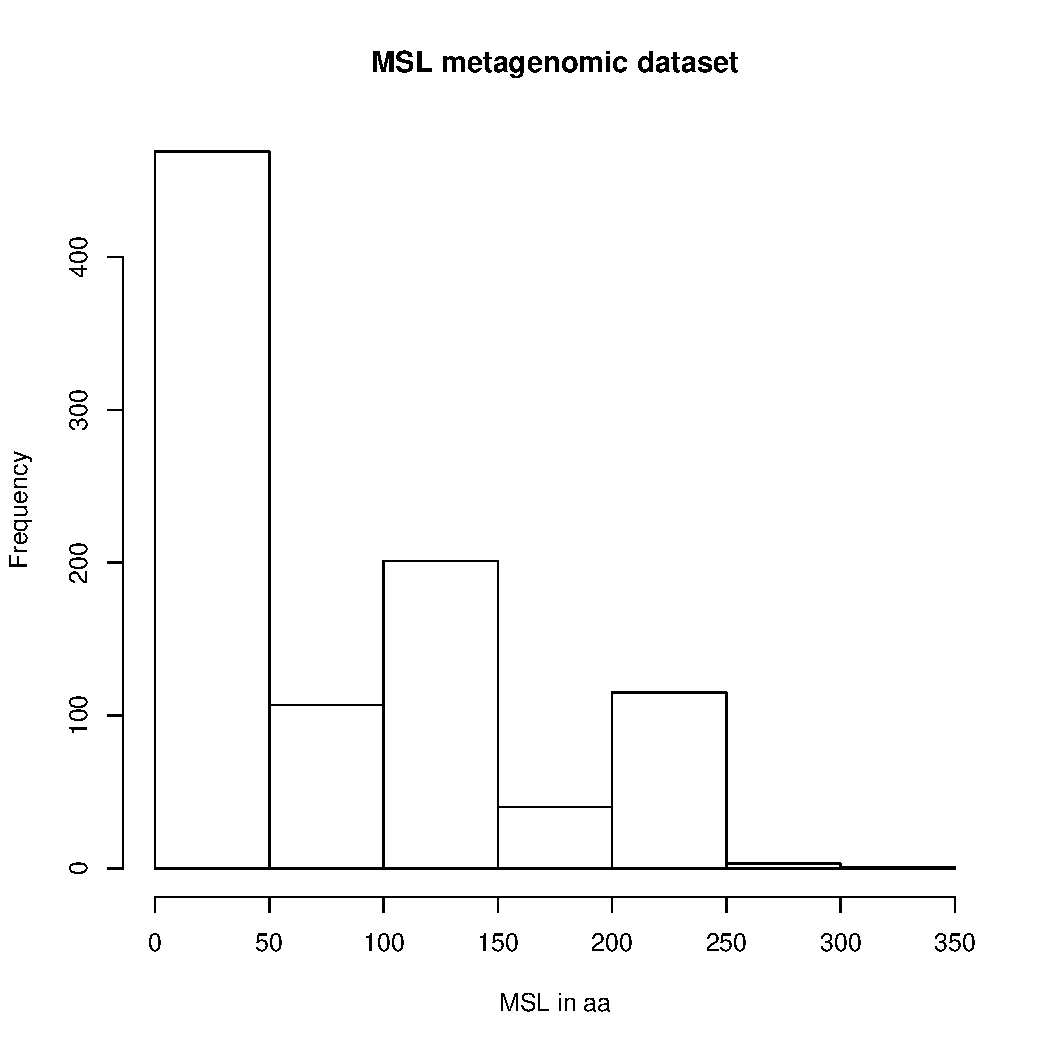
\includegraphics[width=50mm, scale=0.8]{hist.pdf}
    \caption{MSL histogram of the metagenomic dataset }
        \label{fig:msl_metagenomes}
\end{figure}


\section{Stage 2: Domain annotation}
\label{stage2}



\begin{enumerate}
\item Annotate the domain composition of the input proteins (in our case
sucy\_database\_uniprot.fasta) using interproscan and current release of PfamA
(december 2016) 

\begin{verbatim}
/interproscan-5.21-60.0/interproscan.sh -appl PfamA-30.0 
-i /input_data/sucy_database_uniprot.fasta -f tsv -pa 
-iprlookupD
\end{verbatim}

\item  Check the output example, using  following the output information of
\href{https://github.com/ebi-pf-team/interproscan/wiki/InterProScan5OutputFormats}{interproscan}

\begin{verbatim}
less -S sucy_database_uniprot.fasta.tsv
\end{verbatim}

\item To get the markov models of the input  proteins, the following files are
needed

\begin{verbatim}
#1. Complete Pfam database of hmm 
#Get the current realease of Pfam database (heavy file, not provided!)
wget ftp://ftp.ebi.ac.uk/pub/databases/Pfam/current_release/Pfam-A.hmm.gz
gunzip Pfam-A.hmm.gz

\end{verbatim}

\item Get the Specific domain identifiers of the input proteins.Using the output file from interproscan: 
<sucy\_database\_uniprot.fasta.tsv>,  we are interested in the 4th and 5th
column (Analysis and Signature Accession respectively) 

\begin{verbatim}
cut -f 4,5 sucy_database_uniprot.fasta.tsv  > id_interpro.txt 
\end{verbatim}

\item Obtain the specific markov models of the input proteins 

Run the script \textit{extract\_hmms.pl}. 
The latter use as input the  id\_interpro.txt  and the  PfamA.hmm. Make sure
you have those files in the same directory. And the names are exactly the same,
otherwise the script will not work.

\begin{verbatim}
######################
#   Run the script   #
######################

perl ../scripts/extract_hmms.pl 

# Pfam
# hmms = 112 #pfam version 30. Using pfam version 27 we 
obtain a total of  114  hmms  

#This will generate an output file named 'my_Pfam.hmm'. 
(We have compressed the file my_Pfam.hmm.bz2) 
#Note that Superfamily and TIGRFAM HMMs can also be used, 
but are commented out.

\end{verbatim}

\item Annotate Pfam domains in the "omic"-data sets using hmmsearch 

Genomic dataset 
\begin{verbatim}

hmmsearch --cpu 8 --cut_ga -o /dev/null  --tblout 
genomes_refseq_nr_22122016.fa.pf.tab  my_Pfam.hmm 
Gen/genomes_refseq_nr_22122016.1.faa  & 
\end{verbatim}

Genomic dataset (each genome separately) 
Optionally, compute the hmmsearch for each genome to calculate the SScore in
Stage 4, using the same command line  
\begin{verbatim}
nohup for i in /data/GenF/*.faa ; do 
hmmsearch --cpu 8 --cut_ga -o /dev/null --tblout 
$i.out.hmmsearch.tab my_Pfam.hmm  $i; done  & 
\end{verbatim}

Metagenomic dataset  
\begin{verbatim}
nohup for i in /data/Met/* ; do hmmsearch 
--cpu 8 --cut_ga -o /dev/null --tblout 
$i.out.hmmsearch.tab my_Pfam.hmm  $i; done  &
\end{verbatim}

Check the output from the above command in the corresponding directories 

\begin{verbatim}
ls *.tab data/Gen 
ls *.tab data/GenF 
ls *.tab data/Met
\end{verbatim}
\end{enumerate}
\subsection{Pfam domain names}
To get the names of each Pfam, we use the documentation from
\href{https://github.com/Cantalapiedra/pfam_terms}{Cantalapiedra C} 

\begin{verbatim}
Generate a list with the Pfam domains 
cd data/
less entropies_matrix_entropies.tab | cut -f 1 > pfam_terms.tab
Use the script pfam.terms.sh 
cd ../scripts
./pfam.terms.sh 
The latter script will generate this file:
pfam_terms.desc.tab
moved to data directory 
mv pfam_terms.desc.tab ../data/
head pfam_terms.desc.tab 

PF00005	ABC transporter
PF00009	Elongation factor Tu GTP binding domain
PF00034	Cytochrome c
PF00037	4Fe-4S binding domain
PF00106	short chain dehydrogenase
PF00111	2Fe-2S iron-sulfur cluster binding domain
PF00124	Photosynthetic reaction centre protein
PF00171	Aldehyde dehydrogenase family
PF00174	Oxidoreductase molybdopterin binding domain
\end{verbatim}

\section{Stage 3: Relative Entropy}
\label{stage3}

We used a derivative of the Kullback-Leibler divergenc 
(Kullback and Leibler, 1951)—also known as relative entropy 
H’(i)—to measure the difference between two probability 
distributions P and Q (Eq. 1). In this context, P(i) 
represents the total number of occurrences of protein 
family i in sulfur-related genomes (observed frequency), 
while Q(i) represents the total number of occurrences of 
that family in the genomic dataset (expected frequency). 
H’, in bits, captures the extent to which a family informs 
specifically about sulfur metabolism. H’ values that are 
close to 1 correspond to the most informative families 
(enriched among sulfur-related genomes), whereas low H’ 
values (close to zero) describe non-informative families. 
Negative values correspond to protein families observed 
less than expected

%H'= P(i)log2 (aP(i)/Q(i)) #falta poner la ecuación en latex! 

\subsubsection{Requirements to compute relative entropies}
\label{entropies_requirements}
\begin{enumerate}
\item  A hmmsearch TSV outfile with the results of scanning 
a collection of Pfam domais against  a large set of(non-
redundant) genomes (output from hmmsearch in the omic 
datasets )
\item A list of selected accessions of genomes interest to compute entropy (see
input\_data\/suli.nr25122016.txt)
\item An optional list of RefSeq assembly annotations to print scientific names
instead of accession codes (see
\/data\/genomic\_dataset\/assembly\_refseq.nr2016.tx)
\end{enumerate}

Output

\begin{enumerate}

\item A matrix of occurrence of Pfam domains across genomes
\item Entropy estimates of each scanned Pfam domain with respect to the selected accessions
\end{enumerate}

Computing the relative entropy in the genomic and genomic fragmented datasets 

\begin{verbatim}


######################
#Run the script help:#
######################

perl  ../scripts/entropy.pl : usage: ../scripts/entropy.pl 
<pfam_hmmsearch.tab> <accession list (ie Suli)> <RefSeq 
list, optional>

cd data

#GENOMIC DATASET

######################
#   Run the script   #
######################

perl scripts/entropy.pl data/genomic_dataset
/genomes_refseq_nr_22122016.1.faa.out.hmmsearch.tab 
input_data/suli.nr25122016.txt data/genomic_dataset
/assembly_refseq.nr2016.txt  > 
GENOMES_NCBI_nr_28122016_size0_cover0.faa.pf.tab.csv

#GENOMIC FRAGMENTED DATASET  

#genomic fragmented files are not provided, make sure you read 
Stage1.Rmd 

######################
#   Run the script   #
######################

for i in data/genomic_fragmented/*.tab ; do perl 
scripts/entropy.pl $i input_data/suli.nr25122016.txt 
data/genomic_dataset/assembly_refseq.nr2016.txt > $i.csv 

mkdir entropies_matrix
mv *.csv entropies_matrix

\end{verbatim}

\subsubsection{Observing the distribution of the relative entropies}


In order to plot the results obtained with the \textit{entropy.pl} script, the
following scripts are needed:   

\begin{enumerate}

\item  \textit{entropies.py}: The first script requires all the matrix that
contains the relative entropies computed in the genomic and genomic 
fragmented data-set (sizes 30, 60, 100, 150, 200, 250, 
300). The matrix are located in entropies\_matrix 
directory. The scripts  returns a tabular list of the 
entropies. Make sure that the names of the matrix in csv 
format follow this pattern \'\_size([0-9]+)\_\', otherwise 
the script cannot be computed. Besides, all the files need to 
have the same number of domains (profiles) in the same column 
order. This script assumes that these considerations are true, 
so it cannot find errors in the input files format.

\begin{verbatim}

######################
#   Run the script   #
######################

python ../scripts/extract_entropies.py entropies_matrix/

The latter script will generate the following text file 
entropies_matrix__entropies.tab

        real    30      60      100     150     200 ...    
PF00005 -0.001  0.001   -0.001  -0.001  -0.001  -0.001 ...
PF00009 -0.001  -0.014  -0.001  -0.001  -0.001  -0.001 ...
PF00034 -0.119  -0.195  -0.183  -0.153  -0.115  -0.106 ...
\end{verbatim}

\item \textit{plot\_entropy.py}: In order to observe the results of the latter
tabular file, this scripts will generate 5 different plots:
\begin{verbatim}
######################
#Run the script help:#
######################

python3 plot_entropy.py data.tab 

\end{verbatim}

\begin{enumerate}
\item \textbf{entropies\_matrix\_entropies.tab\_bar.png.} Barplot of the
distribution of each Pfam relative entropy, in the different genomic fragmented
sizes. At the top of the figure are the  Pfam's with highest values, and the
bottom are the lowest entropies values . (Figure \ref{fig:barplot})

 \begin{figure}[H]
  \centering
    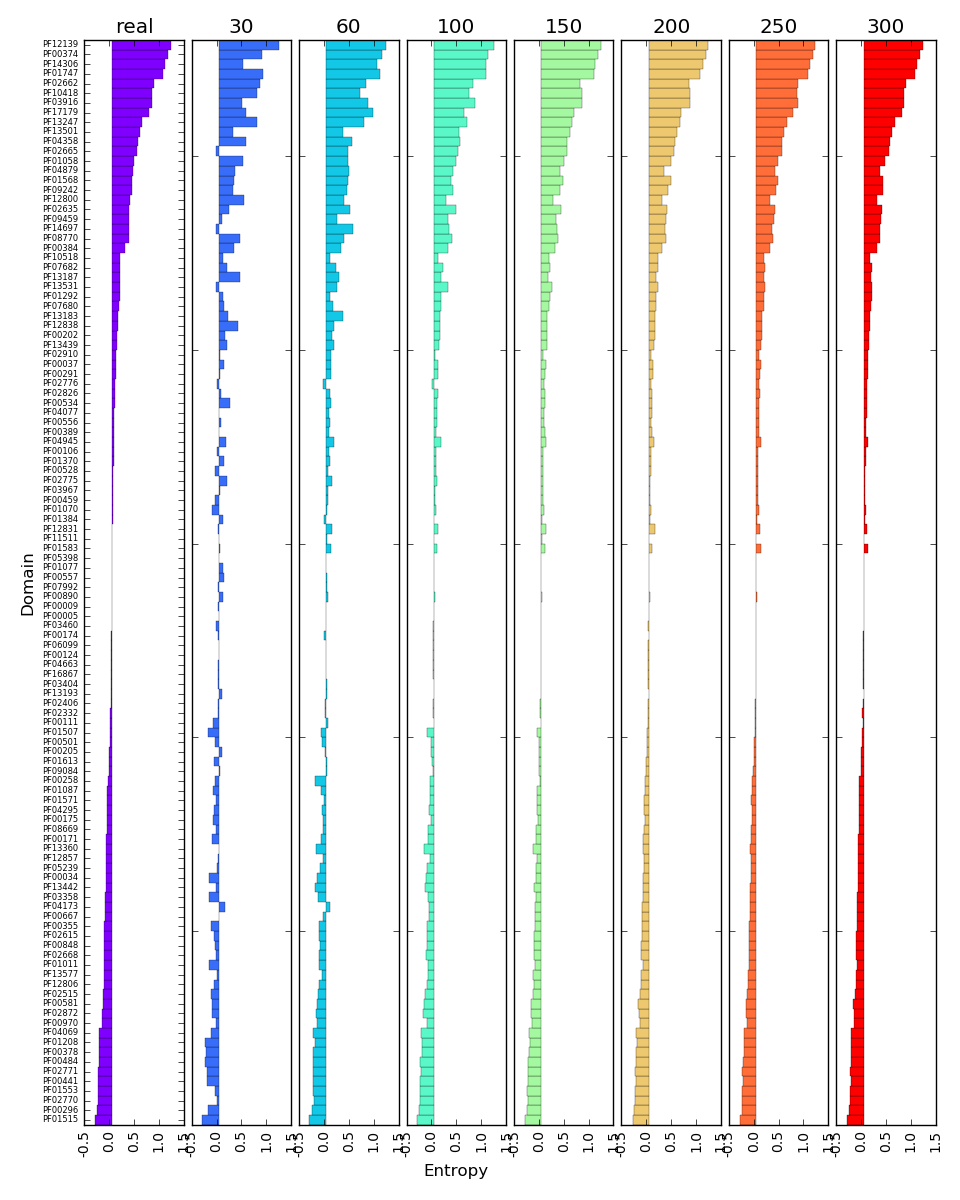
\includegraphics[width=50mm]{entropies_matrix_entropies_tab_bar.png}
    \caption{Barplot }
        \label{fig:barplot}
\end{figure}

\item \textbf{entropies\_matrix\_entropies.tab\_hmap.png}. Heatmap of the
distribution of each Pfam relative entropy, in the different genomic fragmented
sizes. Red values are the highest entropies and blue values the lowest. (Figure
\ref{fig:heatmap})
 \begin{figure}[H]
  \centering
    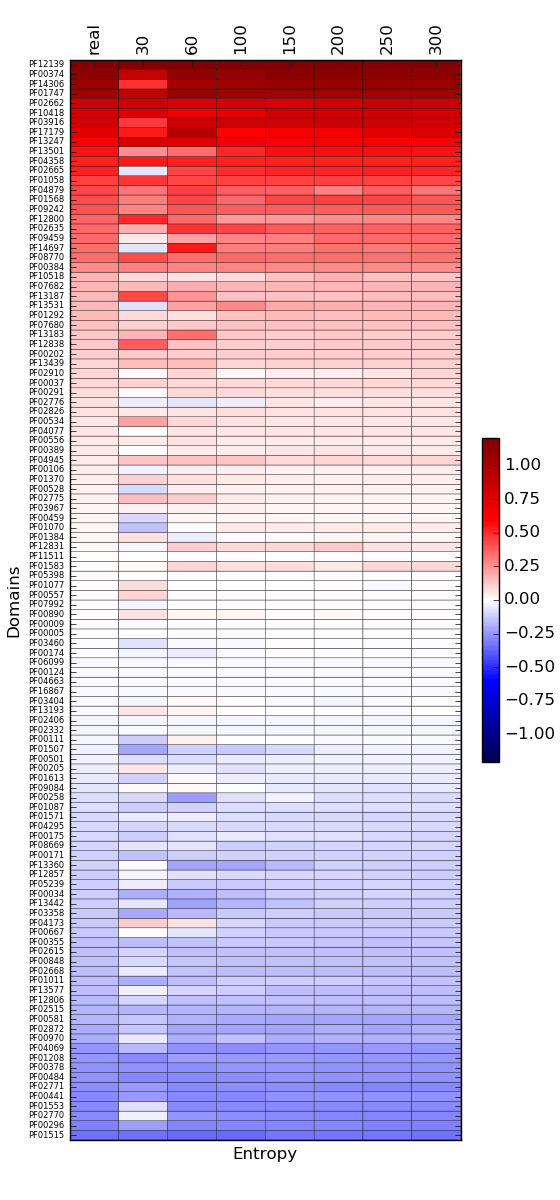
\includegraphics[width=30mm, scale =0.9]{entropies_matrix_entropies_tab_hmap.png}
    \caption{Heatmap plot}
        \label{fig:heatmap}
\end{figure}

\item \textbf{entropies\_matrix\_entropies.tab\_scatter.png}. Scatter plot
showing the mean dispersion of each  Pfam H' (x axis),versus the standard
deviation of the values obtained in the genomic fragmented dataset (y axis). In
this sense the low standard deviation indicates that the H' values are similar
across several datasets of variable sizes, which is useful in the metagenomic
dataset. In this sense, the H' of this specific Pfam's, are not affected by the
size of the metagenome (either read peptides of 30 aa or 300). In the other
hand, high standard deviation indicates that H' is affected by the size. In
this way, high H', and low standard deviation, points the most informative
Pfam's that could be used as molecular marker genes in metagenomes of variable
sizes. (Figure \ref{fig:scatterplot}) 
 \begin{figure}[H]
  \centering
    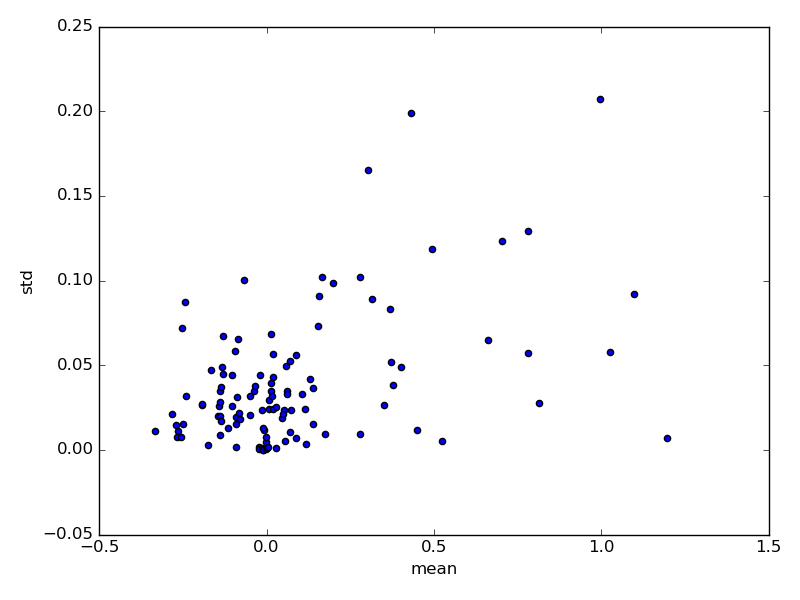
\includegraphics[width=50mm, scale =0.5]{entropies_matrix_entropies_tab_scatter.png}
    \caption{Scatterplot}
        \label{fig:scatterplot}
\end{figure}


\item \textbf{entropies\_matrix\_entropies.tab\_entropy\_hist.png}. Histograms
of the distribution of the H' in the different genomic fragmented sizes.
(Figure \ref{fig:histogram})

\begin{figure}[H]
  \centering
    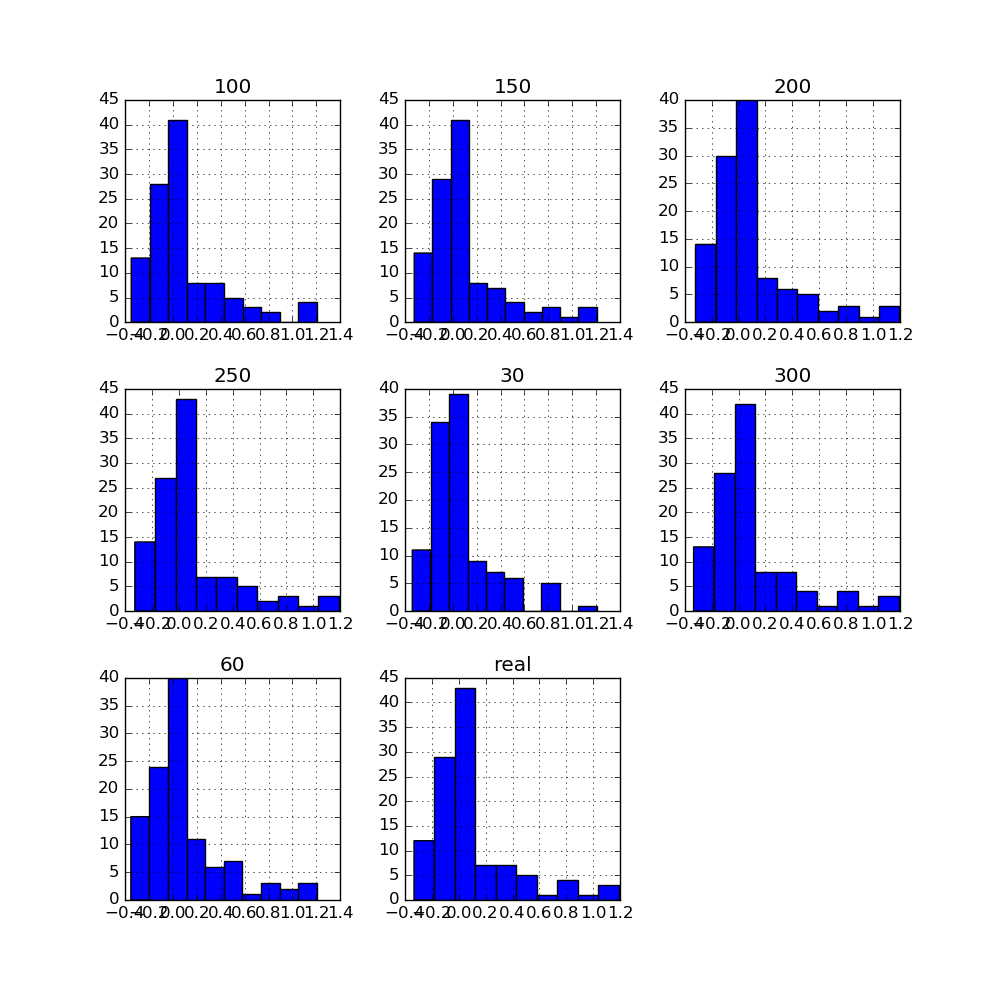
\includegraphics[width=50mm, scale =0.5]{entropies_matrix_entropies_tab_entropy_hist.png}
    \caption{Histogram plot}
        \label{fig:histogram}
\end{figure}

\item \textbf{entropies\_matrix\_entropies.tab\_differential.png}.

Entropy difference of each Pfam H' with respect to real, in order to observe
the degree of change from the previous one. The differential was calculate
along the MSL 

                      \textbf{          $x_i - x_{i-1}$.}

The data was normalized with respect to real values, then the differential was
plotted according to each size (MSL). The highest entropy difference with
respect to real values is obteined in sizes of 30 and 60, indicating that above
this values, the H' of each Pfam are maintained across several datasets of
variable sizes (>60). (Figure \ref{fig:differential})

 \begin{figure}[H]
  \centering
    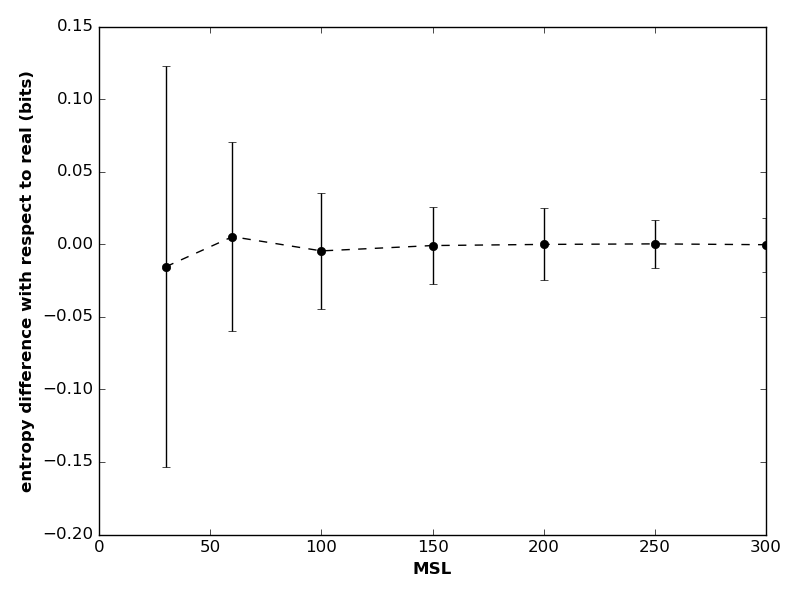
\includegraphics[width=50mm, scale =0.5]{entropies_matrix_entropies_tab_differential.png}
    \caption{Differential plot }
        \label{fig:differential}
\end{figure}

\item \textbf{entropies\_matrix\_entropies.tab\_prof\_box.png}.Boxplot the
distribution of each Pfam relative entropy, in the different genomic fragmented
sizes. Middle blue line indicates cero values. Black lines indicates the
percentile data  (5\% and 95\%) obtained obtained in the random test. (Figure
\ref{fig:boxplot}). See further details in Random entropies.  

\begin{figure}[H]
  \centering
    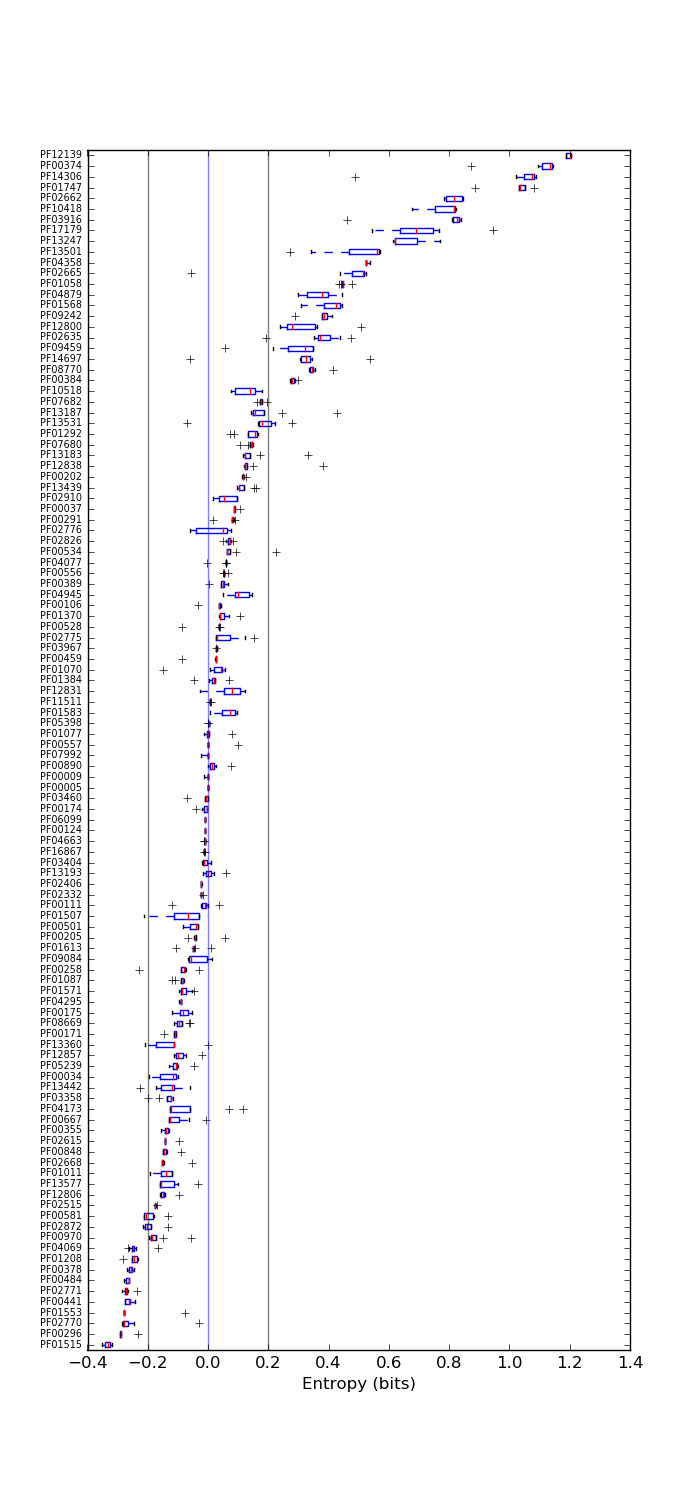
\includegraphics[width=30mm, scale =0.5]{entropies_matrix_entropies_tab_prof_box.png}
    \caption{Boxplot}
        \label{fig:boxplot}
\end{figure}

\subsection{Random entropies}
Due to its nature, the relative entropy might be biased by the 
number of input organisms (in our case sulfur list. For 
this reason, we recalculated H’, this time substituting the S-genomes 
with equally sized lists of random genomes n=161. If there really 
was no such bias, then we could expect to obtain low-informative 
Pfam domains during the random test. 
Using these procedures, we evaluated the variation of relative 
entropy of each Pfam domain in order to short-list those that 
could be used as markers in metagenomic datasets, regardless of 
average length, and to generate a measure to be used as a way to 
compare the importance of sulfur metabolisms in metagenomes 
derived from any environment.
We compute the relative entropies of the same input database of Pfam domains
but using 1000 list of microorganisms (not sulfur based energy). 

Generate the random lists: 
\begin{verbatim}
cd genomic_dataset 
mkdir random_samples 
for ((i=1;i<1001;i+=1)); do cat assembly_refseq.nr2016.txt | 
cut -f 1,8 | shuf -n 161  > random_samples/random$i.txt  ; done

#Compute the random entropy 

#GENOMIC DATASET 
######################
#   Run the script   #
######################
 
for i in random_samples/*.txt; do perl entropy.pl 
genomes_refseq_nr_22122016.1.faa.out.hmmsearch.tab $i 
assembly_refseq.nr2016.txt  > $i.csv ; done 

#GENOMIC FRAGMENTED DATASET 
#(size 30, repeat for each size)

######################
#   Run the script   #
######################

for i in random_samples/*.txt; do perl entropy.pl 
genomes_refseq_nr_22122016_size30_cover10.faa.out.hmmsearch.tab $i   
> $i.30.csv
done

#Extract the entropies of all the 8,000 matrices using the following 
script that will generate a tabular format file of each Pfam and the 
corresponding  H'value in each test (1..100)

######################
#   Run the script   #
######################

perl ../scripts/extract_random_entropies.pl -matrixdir 
random_samples/

# extract_random_entropies.pl call:
# -matrixdir random_samples

# merged file of MSL=real (replicates=1000, random_real.real.tab)

#Generate a new folder and move all the generated files 

mkdir tab_files_random && mv *.tab tab_files_random && mv 
tab_files_random/ .. 

######################
#   Run the script   #
######################

python3 ../scripts/plot_random_entropies.py random_real.real.tab 

#The script will generate three different outputs. 

1) Percentile distribution at 5% and 95%  of each Pfam H',  in the 
1000 random matrices, for example:

PF13501  5-percentile= -0.049  95-percentile= 0.077
PF13531  5-percentile= -0.058  95-percentile= 0.058

2) The total min 5-percentile and max 95-percentile 
# min  5-percentile= -0.091
# max 95-percentile= 0.101

3)Boxplot distribution of each Pfam H', indicating the lines of the 
max an min percentile distribution. 
\end{verbatim}

Using the above mentioned script, we obtained both: 1) the percentile data of
all the tabular files computed for each size (MSL) (Table \ref{percent}), and
2) the boxplot distribution of each  Pfam H' value in the the random
test(Figure \ref{fig:cutoff_random}). 


\begin{table}[]
\centering
\caption{min 5 and max 95 percentile distribution of Pfam's H' in each MSL}
\label{percent}
\begin{tabular}{@{}ccc@{}}
\toprule
MSL  & 5 percentile & 95 percentile \\ \midrule
Real & -0.091       & 0.101         \\
30   & -0.086       & 0.105         \\
60   & -0.09        & 0.105         \\
100  & -0.088       & 0.1           \\
150  & -0.09        & 0.103         \\
200  & -0.089       & 0.105         \\
250  & -0.09        & 0.106         \\
300  & -0.09        & 0.1             \\ \bottomrule
\end{tabular}
\end{table}



\end{enumerate}
\end{enumerate}

As observed in Table \ref{percent}, the data obtained is symmetric, indicating
that the Pfam H' that fall into this values  (-0.1 and 0.01), are more likely
to be obtained randomly, therefore the higher values (>0.01), are really
informative Pfam's. 
Then, we use two more strict cut off values for min and max percentiles (-0.2,
0.2 and -0.3, 0.3) in order to excluded all the Pfam H' that are observed in
the random test. Using this criteria, is observed that some Pfam's including
within this range (blue boxes in Figure \ref{fig:cutoff_random} ) are lost
using the strict criteria. In our case we decided to use the percentile
distribution obtained with the random test (-0.1 and 0.1), to observe those
informative (higher H'), and those under-informative (lower H'). In the latter
case, this Pfam's indicates that almost non sulfur based microorganisms posses
this gene family.  

\begin{figure}[H]
  \centering
    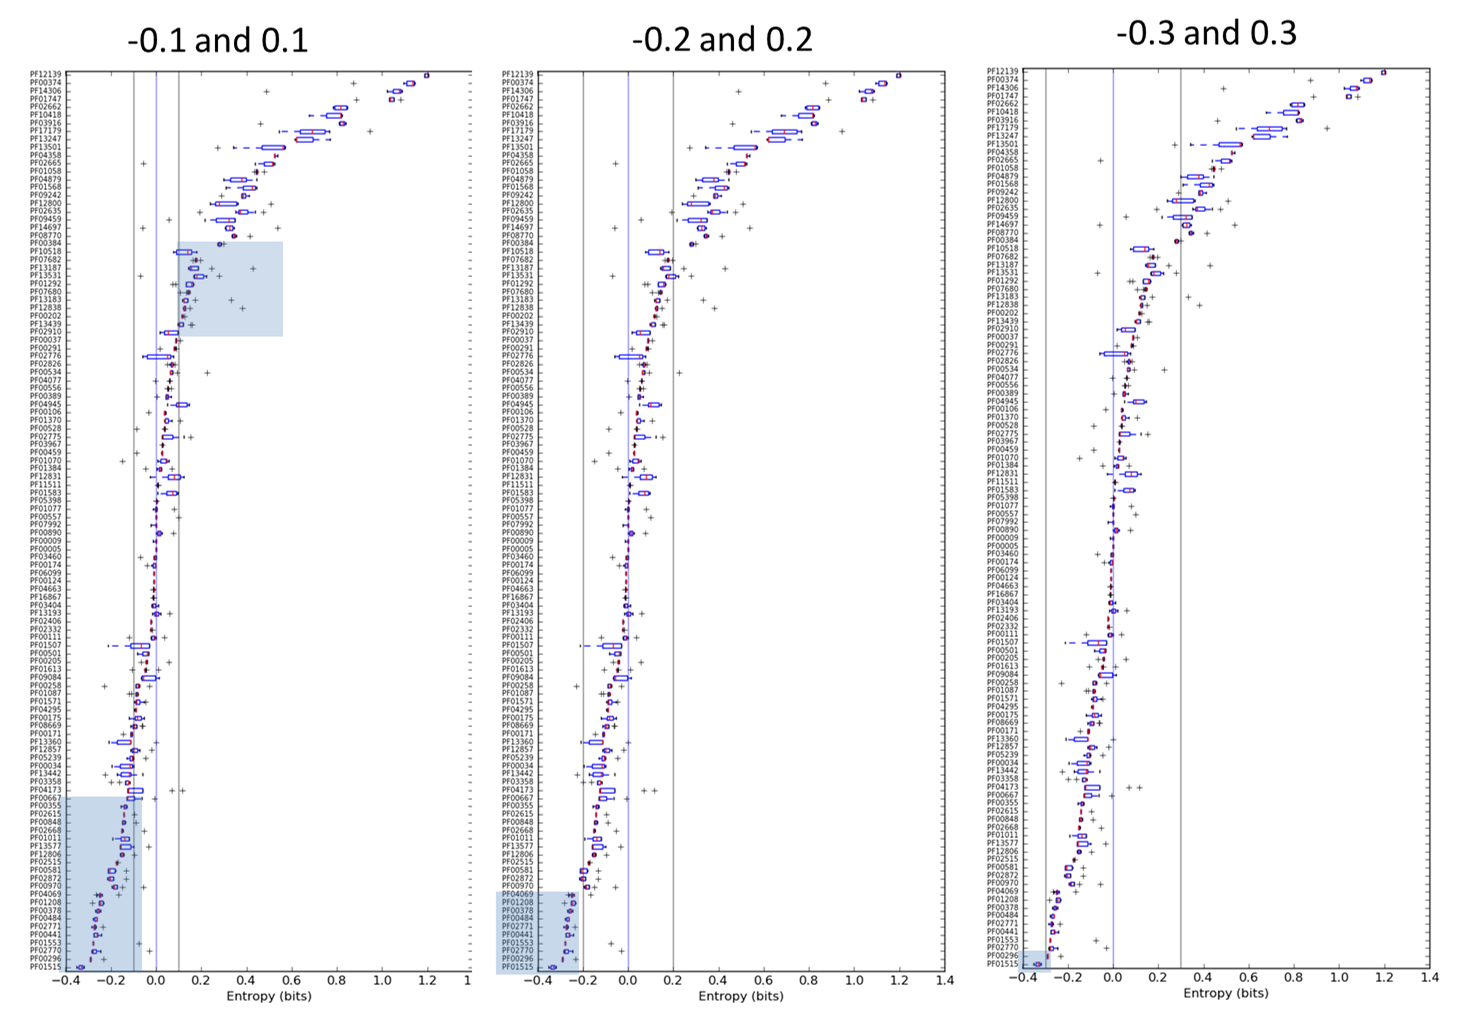
\includegraphics[width=100mm, scale =0.8]{cutoff_random.png}
    \caption{Different cutoff values for min 5 and max 95 percentile values}
        \label{fig:cutoff_random}
\end{figure}

\subsection{Informative Pfam's:Molecular marker genes in metagenomic data}

In order to benchmark the behavior of Pfam´s H' in metagenomic dataset, we
identify those protein families that regardless of the size of the mean size
length (MSL) of the genomic fragemented dataset,   have a consistently high H’
values (H'>=1 bit)  and low standard deviation (std). In order to observe the
behavior of the data, we conducted a clustering analysis 

Before running the script, make sure you have installed all dependency modules 
\begin{verbatim}

#######################
# Python Dependencies #
#######################

sudo apt-get install python3-pip
pip3 install -U scikit-learn

#The script was modified from http://scikit-learn.org/stable
/modules/clustering.html#clustering

cd data/clustering

######################
#   Run the script   #
######################

python3 ../../plot_cluster_comparison.py ../entropies_matrix_entropies.tab
\end{verbatim}

Analyze the Figure \ref{fig:cluster_comparision} and observe the behavior of
the data in the last row. In our case Ward and Birch clustering methods
separate in different clusters the Pfam's H' with low std and high H'. 
\begin{verbatim}

cd data/clustering

######################
#   Run the script   #
######################

python3 ../../scripts/F_meanVSstd.py  
../entropies_matrix_entropies.tab -o entropies_matrix_cluster.png  
\end{verbatim}

 \begin{figure}[H]
  \centering
    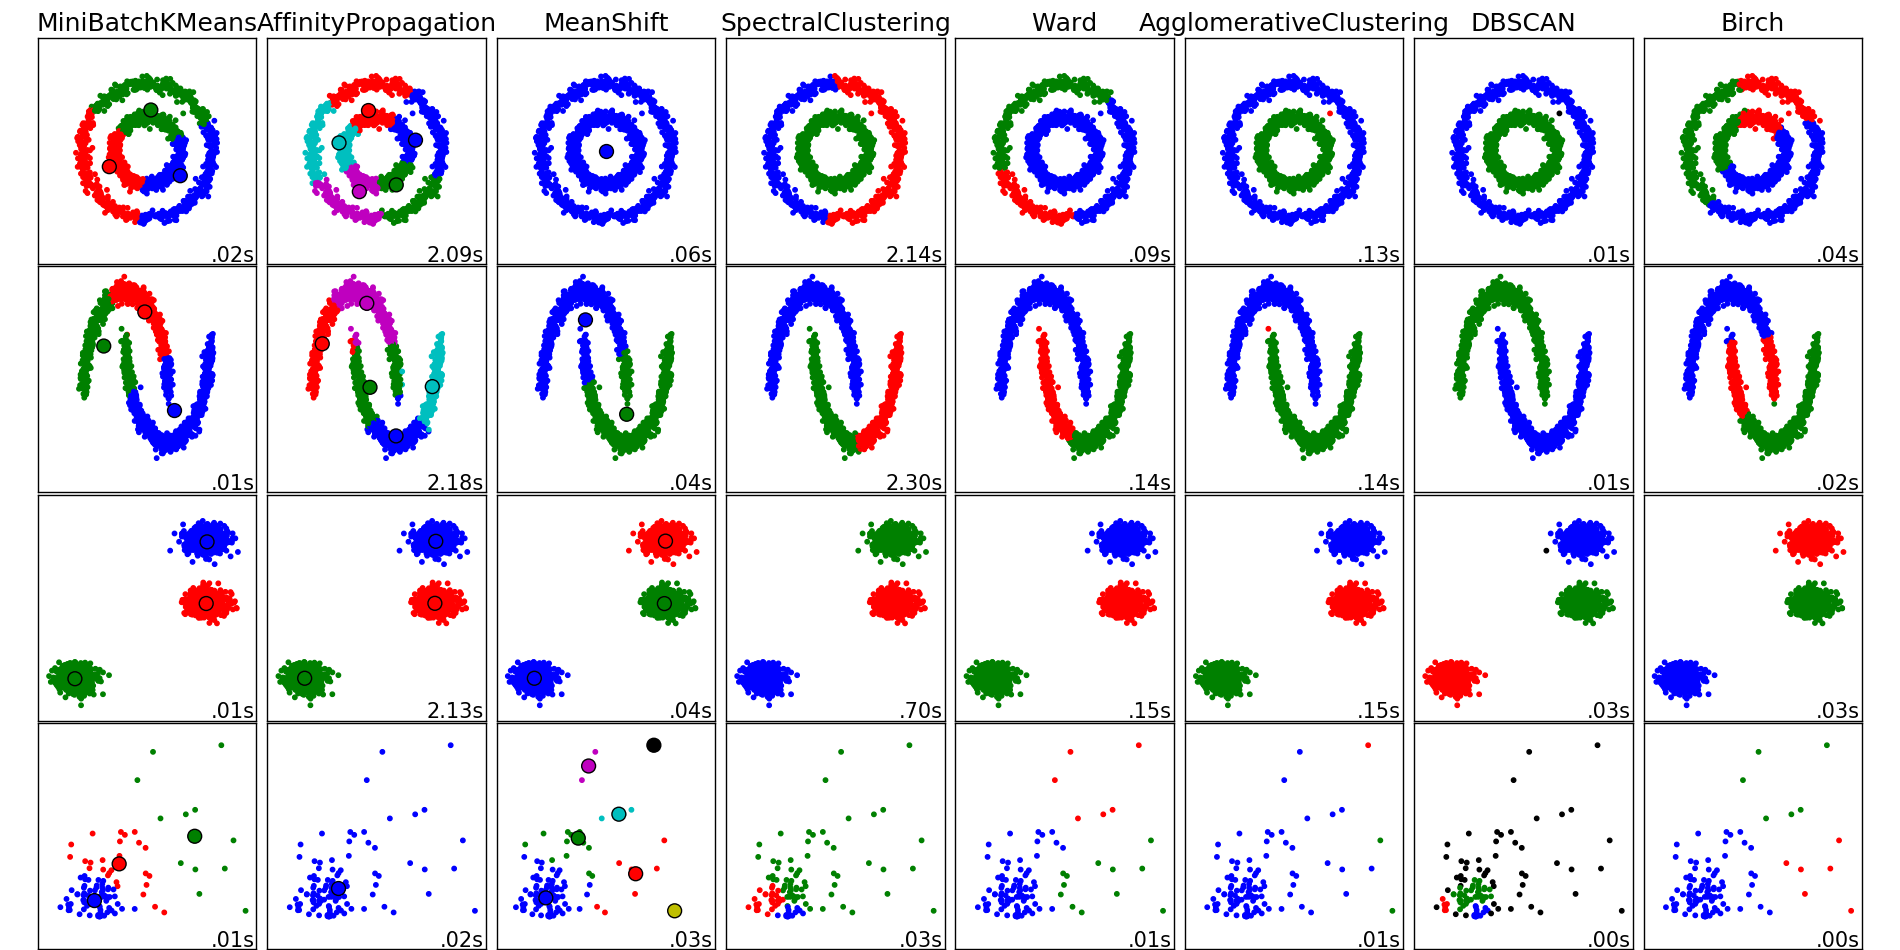
\includegraphics[width=100mm, scale=1]{entropies_matrix_entropies_tab_cluster_comparision.png}
    \caption{Cluster comparision}
        \label{fig:cluster_comparision}
\end{figure}

In order to observe the behavior of each Pfam H', we generate the script
\textit{F\_meanVSstd.py}. Which have several options: 
\begin{verbatim}
######################
#Run the script help:#
######################

python3 scripts/F_meanVSstd.py -h 
usage: F_meanVSstd.py [-h] [-o OUT_FIG] [--dpi DPI] [-v {std,cv,id,range}]
                      [-k {2,3,4,5,6,7,8}] [--plot-random DIRECTORY]
                      [-c {ward,birch}] [--labels CLUSTER]
                      filename

Mean vs standard deviation figure of profiles and clustering. Creates a file
for each cluster that contains the list of profiles that are included.

positional arguments:
  filename              Input file in tabular format. Rows are pfam families
                        and columns are metagenome fragment (reads) length.

optional arguments:
  -h, --help            show this help message and exit
  -o OUT_FIG, --out_fig OUT_FIG
                        Stores the figure in the specified file (and format).
  --dpi DPI             Resolution for output figure file [300].
  -v {std,cv,id,range}, --variation {std,cv,id,range}
                        Select the measurement of variation to plot in y axis
                        [std]: standard devitation (std), coefficient of
                        variation (cv), index of dispersion (id) or range. cv
                        and id cannot be used in variables with negative
                        values.
  -k {2,3,4,5,6,7,8}    Number of k-means clusters [3].
  --plot-random DIRECTORY
                        Folder where the *.tab files containing random samples
                        are stored.
  -c {ward,birch}, --cluster-alg {ward,birch}
                        Chose clustering algorithm [ward]. Ward linked
                        hierarchical clustering or birch clustering.
  --labels CLUSTER      Plot the labels of the points in the specified
                        cluster.
\end{verbatim}
\subsubsection{Basic clustering}
\begin{verbatim}
cd data/clustering

######################
#   Run the script   #
######################

python3 ../../scripts/F_meanVSstd.py ../entropies_matrix_entropies.tab -o 
entropies_cluster.basic.png

#The latter command executes the default script 
parameters (ward cluster, k=3), and std as measurement of 
variation. The output files are the following :
1) Figure: entropies_cluster.basic.png
2) Tabular format file containing the data of first cluster: 
cluster_0_std_k3_ward.tab
3) Tabular format file containing the data of the second cluster 
cluster_1_std_k3_ward.tab
4) Tabular format file contaninig the data of the third cluster. 
cluster_2_std_k3_ward.tab
\end{verbatim}
\begin{figure}[H]
  \centering
    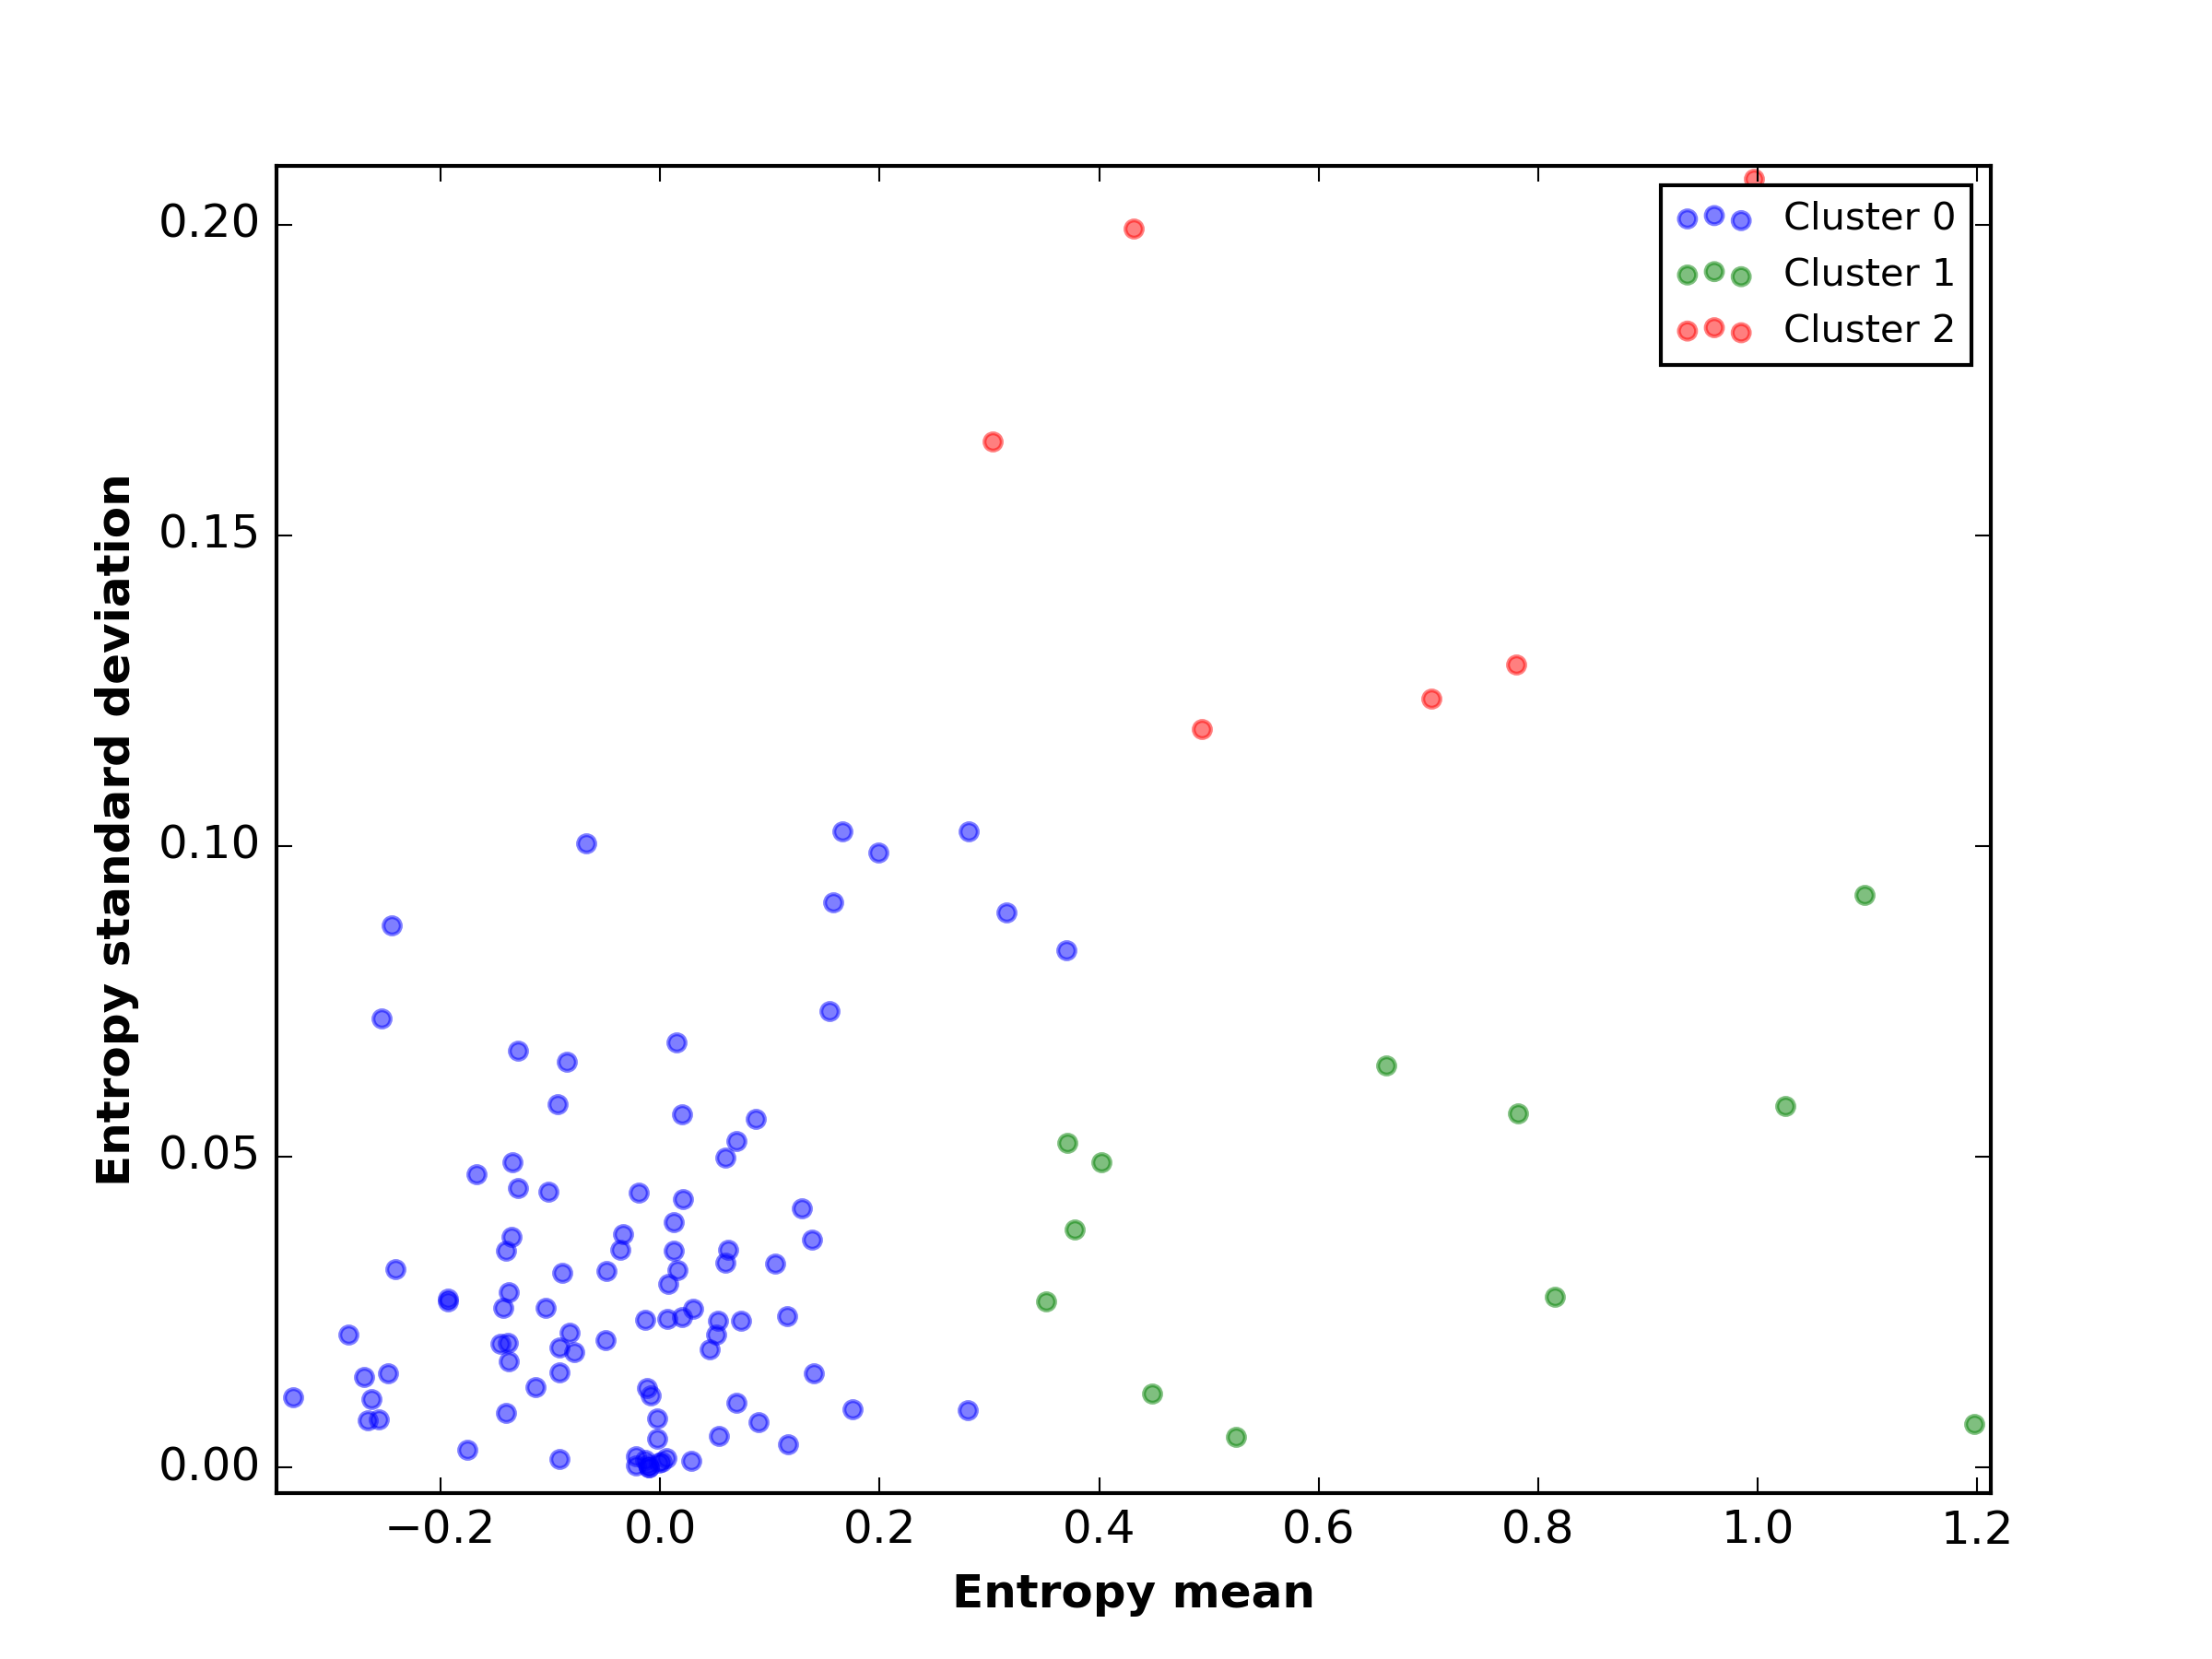
\includegraphics[width=70mm, scale=1]{entropies_cluster_basic.png}
    \caption{Basic usage script F\_meanVSstd.py}
        \label{fig:cluster_basic}
\end{figure}

\subsubsection{Comparing  the distribution of random entropies}

In order to compare the variation of the distribution of the Pfam's H' in the
random test (as observed also in Figure \ref{fig:cutoff_random}),the script
will read the tabular files derived from the random test and will perform the
same analysis (clustering and variation measurements) 
\begin{verbatim}
cd data/clustering

######################
#   Run the script   #
######################

python3 ../../scripts/F_meanVSstd.py  ../entropies_matrix_entropies.tab 
--plot-random  ../tab_files_random/ --labels 1 
-o entropies_cluster_random.png

\end{verbatim}
\begin{figure}[H]
  \centering
    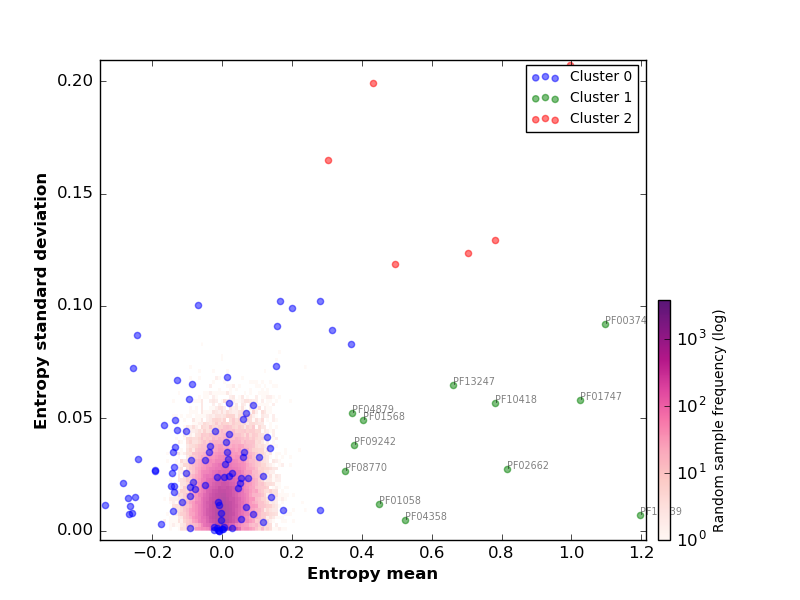
\includegraphics[width=70mm, scale=1]{entropies_random_labels.png}
    \caption{Comparing random distribution}
        \label{fig:cluster_random}
\end{figure}

\subsubsection{Comparing the distribution of random entropies, other
measurement of variation and several clusters}
Using several number of clusters and changing the variation measurement to
observe the data variation. 

\begin{verbatim}
######################
#   Run the script   #
######################

python3 ../../scripts/F_meanVSstd.py  ../entropies_matrix_entropies.tab 
--plot-random ../tab_files_random/ -v range -k 6
--labels 2 -o entropies_cluster_random.range.k6.png


\end{verbatim}
\begin{figure}[H]
  \centering
    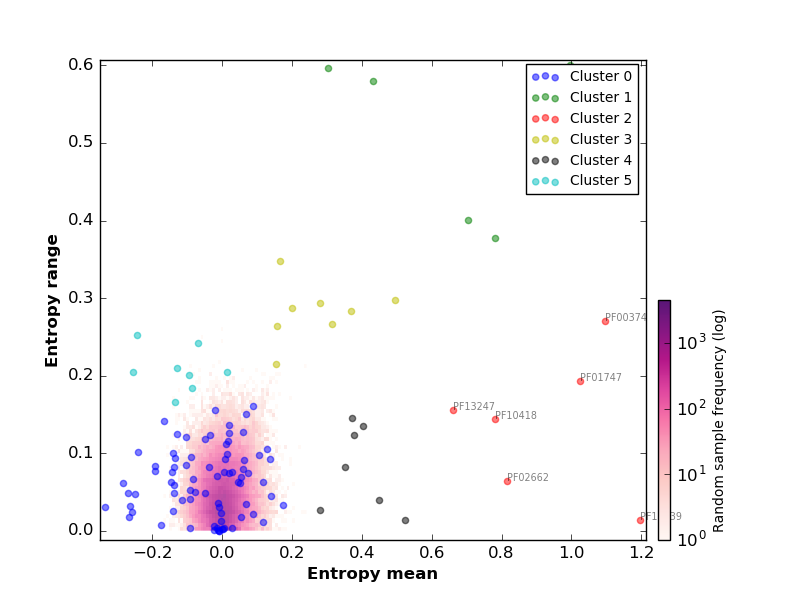
\includegraphics[width=70mm, scale=1]{entropies_cluster_random_range_k6.png}
    \caption{Comparing random distribution, range as measurement of variation and k=6}
        \label{fig:range_random}
\end{figure}

The criteria to select the cluster method to stand out the Pfam’s to benchmark
the metagenomic dataset,  most be based in the distribution of the H’ values
obtained in the random test and biochemical knowledge. Due to the consistence
in the data, we select ward method, k=3 and standard deviation as variation
measurement. 

\section{Stage 4: Entropy Score, origin and interpretation}

\subsection{Requirements}

Due to the variation in peptide read size among the metagenomic dataset (see
Figure \ref{fig:msl_metagenomes}, it will be computationally exhaustive to
fragment the genomic dataset in all the observed sizes. Therefore we choose to
fragment the dataset according to the observed sizes in the histogram:
30,60,100,150,200,250,300 (Figure \ref{fig:msl_metagenomes}). Taking this into
account, we propose a range of (+-) 15 aminoacids above or below the size to
compute the Sscore. In this case, the Score of  a metagenome of MSL of 40 will
be computed using the pre-computed entropies of the genomic fragmented dataset
of size 30. See Table \ref{MSL-input}

\begin{table}[H]
\centering
\caption{MSL selection of input metagenome}
\label{MSL-input}
\begin{tabular}{@{}lll@{}}
\toprule
Details             & GenF size & MSL     \\ \midrule
nr-genomes size 30  & 30        & 0-45    \\
nr-genomes size 60  & 60        & 45-80   \\
nr-genomes size 100 & 100       & 80-125  \\
nr-genomes size 150 & 150       & 125-175 \\
nr-genomes size 200 & 200       & 175-225 \\
nr-genomes size 250 & 250       & 225-275 \\
nr-genomessize 300  & 300       & 275-300 \\ \bottomrule
\end{tabular}
\end{table}

If you want to compute the Score selecting entropies of a certain 
size (H'>=1), you can select this 
option, however  the higher the number chosen for the entropy,  
the less informative the SS will be in terms of importance of 
global biogeochemical cycles. Therefore, we strongly recommend to 
use specific Pfam's rather than entropy cut-off. 

\subsection{Computing the score}
\label{entropy_score}
\begin{verbatim}
######################
#Run the script help:#
######################

perl pfam_score.pl
usage: pfam_score.pl [options] 
 -help             brief help message
-input            input file with HMM matches created by 
hmmsearch, tbl format
 -size             desired size for produced random 
 fragments    (integer, default 100)
  -bzip             input file is bzip2-compressed
-matrixdir        directory containing hmm matrices from 
fragments of variable size (string, 
                    default /data/matrix)
-minentropy       min relative entropy of HMMs to be considered (float)
 -keggmap          file with HMM to KEGG mappings
-pathway          comma-separated pathway numbers from -keggmap 
file to consider only member HMMs  (string, by default all 
pathways are used, requires -keggmap)
\end{verbatim}
\subsubsection{Basic Usage }

\begin{enumerate}
\item Locate the output files from hmmsearch of the metagenomes of interest
(tabular format files). 
\item Locate the matrix folder of the computed entropies in Stage
\ref{entropies_requirements} 
\item Select the desirable MSL size according to Table \ref{MSL-input}
\end{enumerate}
\begin{verbatim}
cd data/metagenomic_dataset
#Single metagenome Score 
#The example metagenome  4546294.3 has a MSL of 30, therefore 
the adecuate Score is 30

######################
#   Run the script   #
######################

perl ../../scripts/pfam_score.pl -input 4546294.3.hmmsearch.tab 
-size 30 -matrixdir ../entropies_matrix/  

# ../../scripts/pfam_score.pl call:
# -input 4546294.3.hmmsearch.tab -size 30 -bzip 0 -matrixdir 
../entropies_matrix/ -minentropy 0 -keggmap  -pathway 
# total HMMs with assigned entropy in ../entropies_matrix
//genomes_refseq_nr_22122016_size30_cover10.faa.out.hmmsearch.tab.csv : 112
PF00005 0.001   1425
PF00009 -0.014  0
PF00034 -0.195  0
PF00037 0.107   212
..........
Pfam entropy score: 12.396
\end{verbatim}
\subsubsection{SS in the metagenomic dataset}

In the case of the example above (metagenome 4546294.3) the SS is 12.396. In
order to benchmark the behavior of the SS in the metagenomic dataset (using all
the described sizes), use the following bash command. 

\begin{verbatim}
#Generate a folder containing all the outputs from hmmsearch and 
move all the tab files  
cd data/metagenomic_dataset
mkdir output_hmmsearch && mv *.hmmsearch.tab output_hmmsearch && 
cd output_hmmsearch 

######################
#   Run the script   #
######################

for file in *.tab; do perl ../../scripts/pfam_score.pl -input 
$file -size 30  -matrixdir ../data/entropies_matrix/  > 
$file.30.score ; done 

#Repeat this command changing -size and the output name. 

#Extract the score of all the metagenomes using grep and 
sed. The regex will depend on the name of your output name 
from hmmsearch. i.e:

grep "Pfam entropy score:" *.score | sed 's/:/\t/g' > 
total.scores.csv 

#The easy way to obtain a tabular format file containing all the 
metagenomes (rows) and their corresponding Scores in all the 
selected sizes (MSL) is using a pivot table implemented in python, excel or libreoffice.

#Check the tabular file output_all_scores.tab  as an example 
less output_all_scores.tab

#To observe the differential plots, open in your browser the 
file differential_plots.html

#Or  you can use the notebook to run each step.

#######################
# Python Dependencies #
#######################

sudo apt-get install build-essentials python-dev python3-dev
sudo apt-get install ipython-notebook ipython3-notebook
sudo pip install -U ipython
sudo pip3 install -U ipython
sudo pip3 install -U jupyter

Once installed all the dependencies, you can use the 
notebook, using the following command line:

ipython3 notebook differential_plots.ipynb

\end{verbatim}
\subsection{Score variation in the metagenomic dataset }

The behavior of the Score in the metagenomic dataset is observed in Figure
\ref{fig:differential}, were the MSL category ("x" axis) is plotted against the
differential ("y" axis). The differential is defined as degree of change of one
size category respect to the previous one ($x_i - x_{i-1}$).
\href{https://docs.scipy.org/doc/numpy/reference/generated/numpy.diff.html}{numpy-python}.
Using this equation, it is possible to observe the variation of the SS computed
for each metagenome in the several MSL categories.We observe that the greatest
difference is obtained in size 30-60 (highest standard deviation). The latter
suggest that  
\begin{enumerate}
\item In metagenomes with MSL of 100-300, the SS can be computed considering
sizes >100 as input for the algorithm. 
\item In small metagenomes (<60), the SS has to be accurately computed, taking into account the specific size of the metagenome.
\end{enumerate} 
Due to the above, we decided to compute the SS of each metagenome according to
the MSL to consider the specific input size.   


\begin{figure}[H]
  \centering
    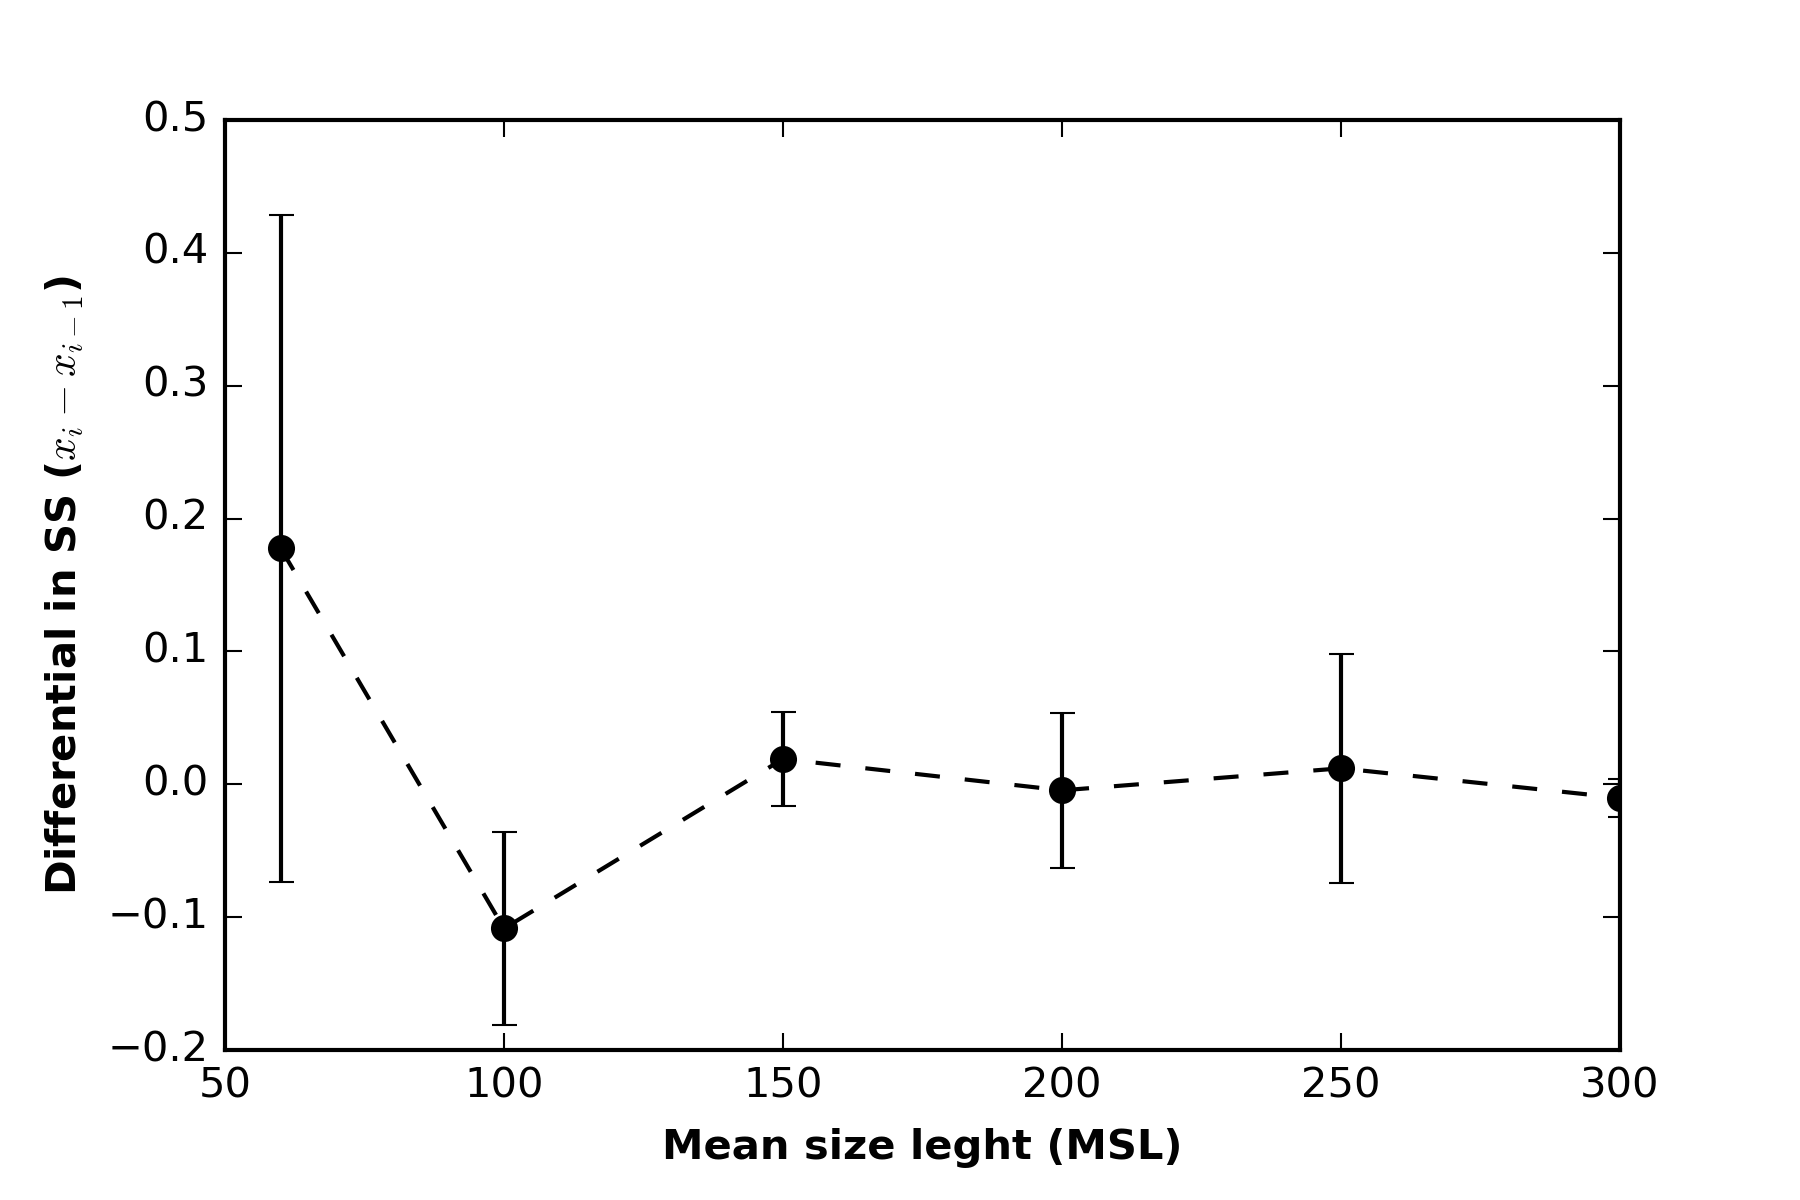
\includegraphics[width=100mm, scale =0.5]{Score_data_behaviour7.png}
    \caption{Degree of change of SS in the metagenomic dataset }
        \label{fig:differential}
\end{figure}

\subsection{Evaluation of the score and the metagenomic metadata}
  
Using the public information derived from each metagenome, it is possible to
obtain the geographical localization of each environmental sample with their
corresponding Pfam Score. 
First, we need to download the meta data and compile some python dependencies
 
\begin{verbatim}
#######################
# Python Dependencies #
#######################

sudo apt-get install python3-mpltoolkits.basemap

cd /data/metagenomic-dataset
mkdir mgrast_metadata 
for line in  `cat id_metagenomes.txt`;  do wget 
"http://api.metagenomics.anl.gov/1/metagenome/mgm$line?verbosity=metadata" 
-O $line ; done 
\end{verbatim}
The latter command will download all the metadata associated to each metagenome
in json format ( http://json.org/).

Then, use the script \textit{create\_metadata\_table.py} to generate a readable
table were each row corresponds to one metagenome and their corresponding
columns represent the metadata associated. 
 
\begin{verbatim}
######################
#Run the script help:#
######################

python3 scripts/create_metadata_table.py -h

usage: create_metadata_table.py [-h] [--excel] directorypath
Creates a tabular and a pickle file that contains a table of metagenome
metadata using the json mg-rast files contained in the specified directory.
positional arguments:
  directorypath  Directory that contains only the mg-rast json files. Each
                 file corresponds to one metagenome.
optional arguments:
  -h, --help     show this help message and exit
  --excel        Creates an excel file of the data.
######################
#   Run the script   #
######################

python3 /scripts/create_metadata_table.py mgrast-metadata/ 

#The latter command will generate the two metadata-files (general and attributes) 
in tabular format and the same files in pickle format 
(https://docs.python.org/2/library/pickle.html):
1) generaldata.tab  and _generaldata.pk
2) attributes.tab and attributes.pk   
 
\end{verbatim}

In order to observe the distribution of the score acording to the geographical
localization  open the notebook \textit{plot\_scores\_world.ipynb} 
\begin{verbatim}
ipython3 notebook plot_scores_world.ipynb
\end{verbatim}

\begin{figure}[H]
  \centering
    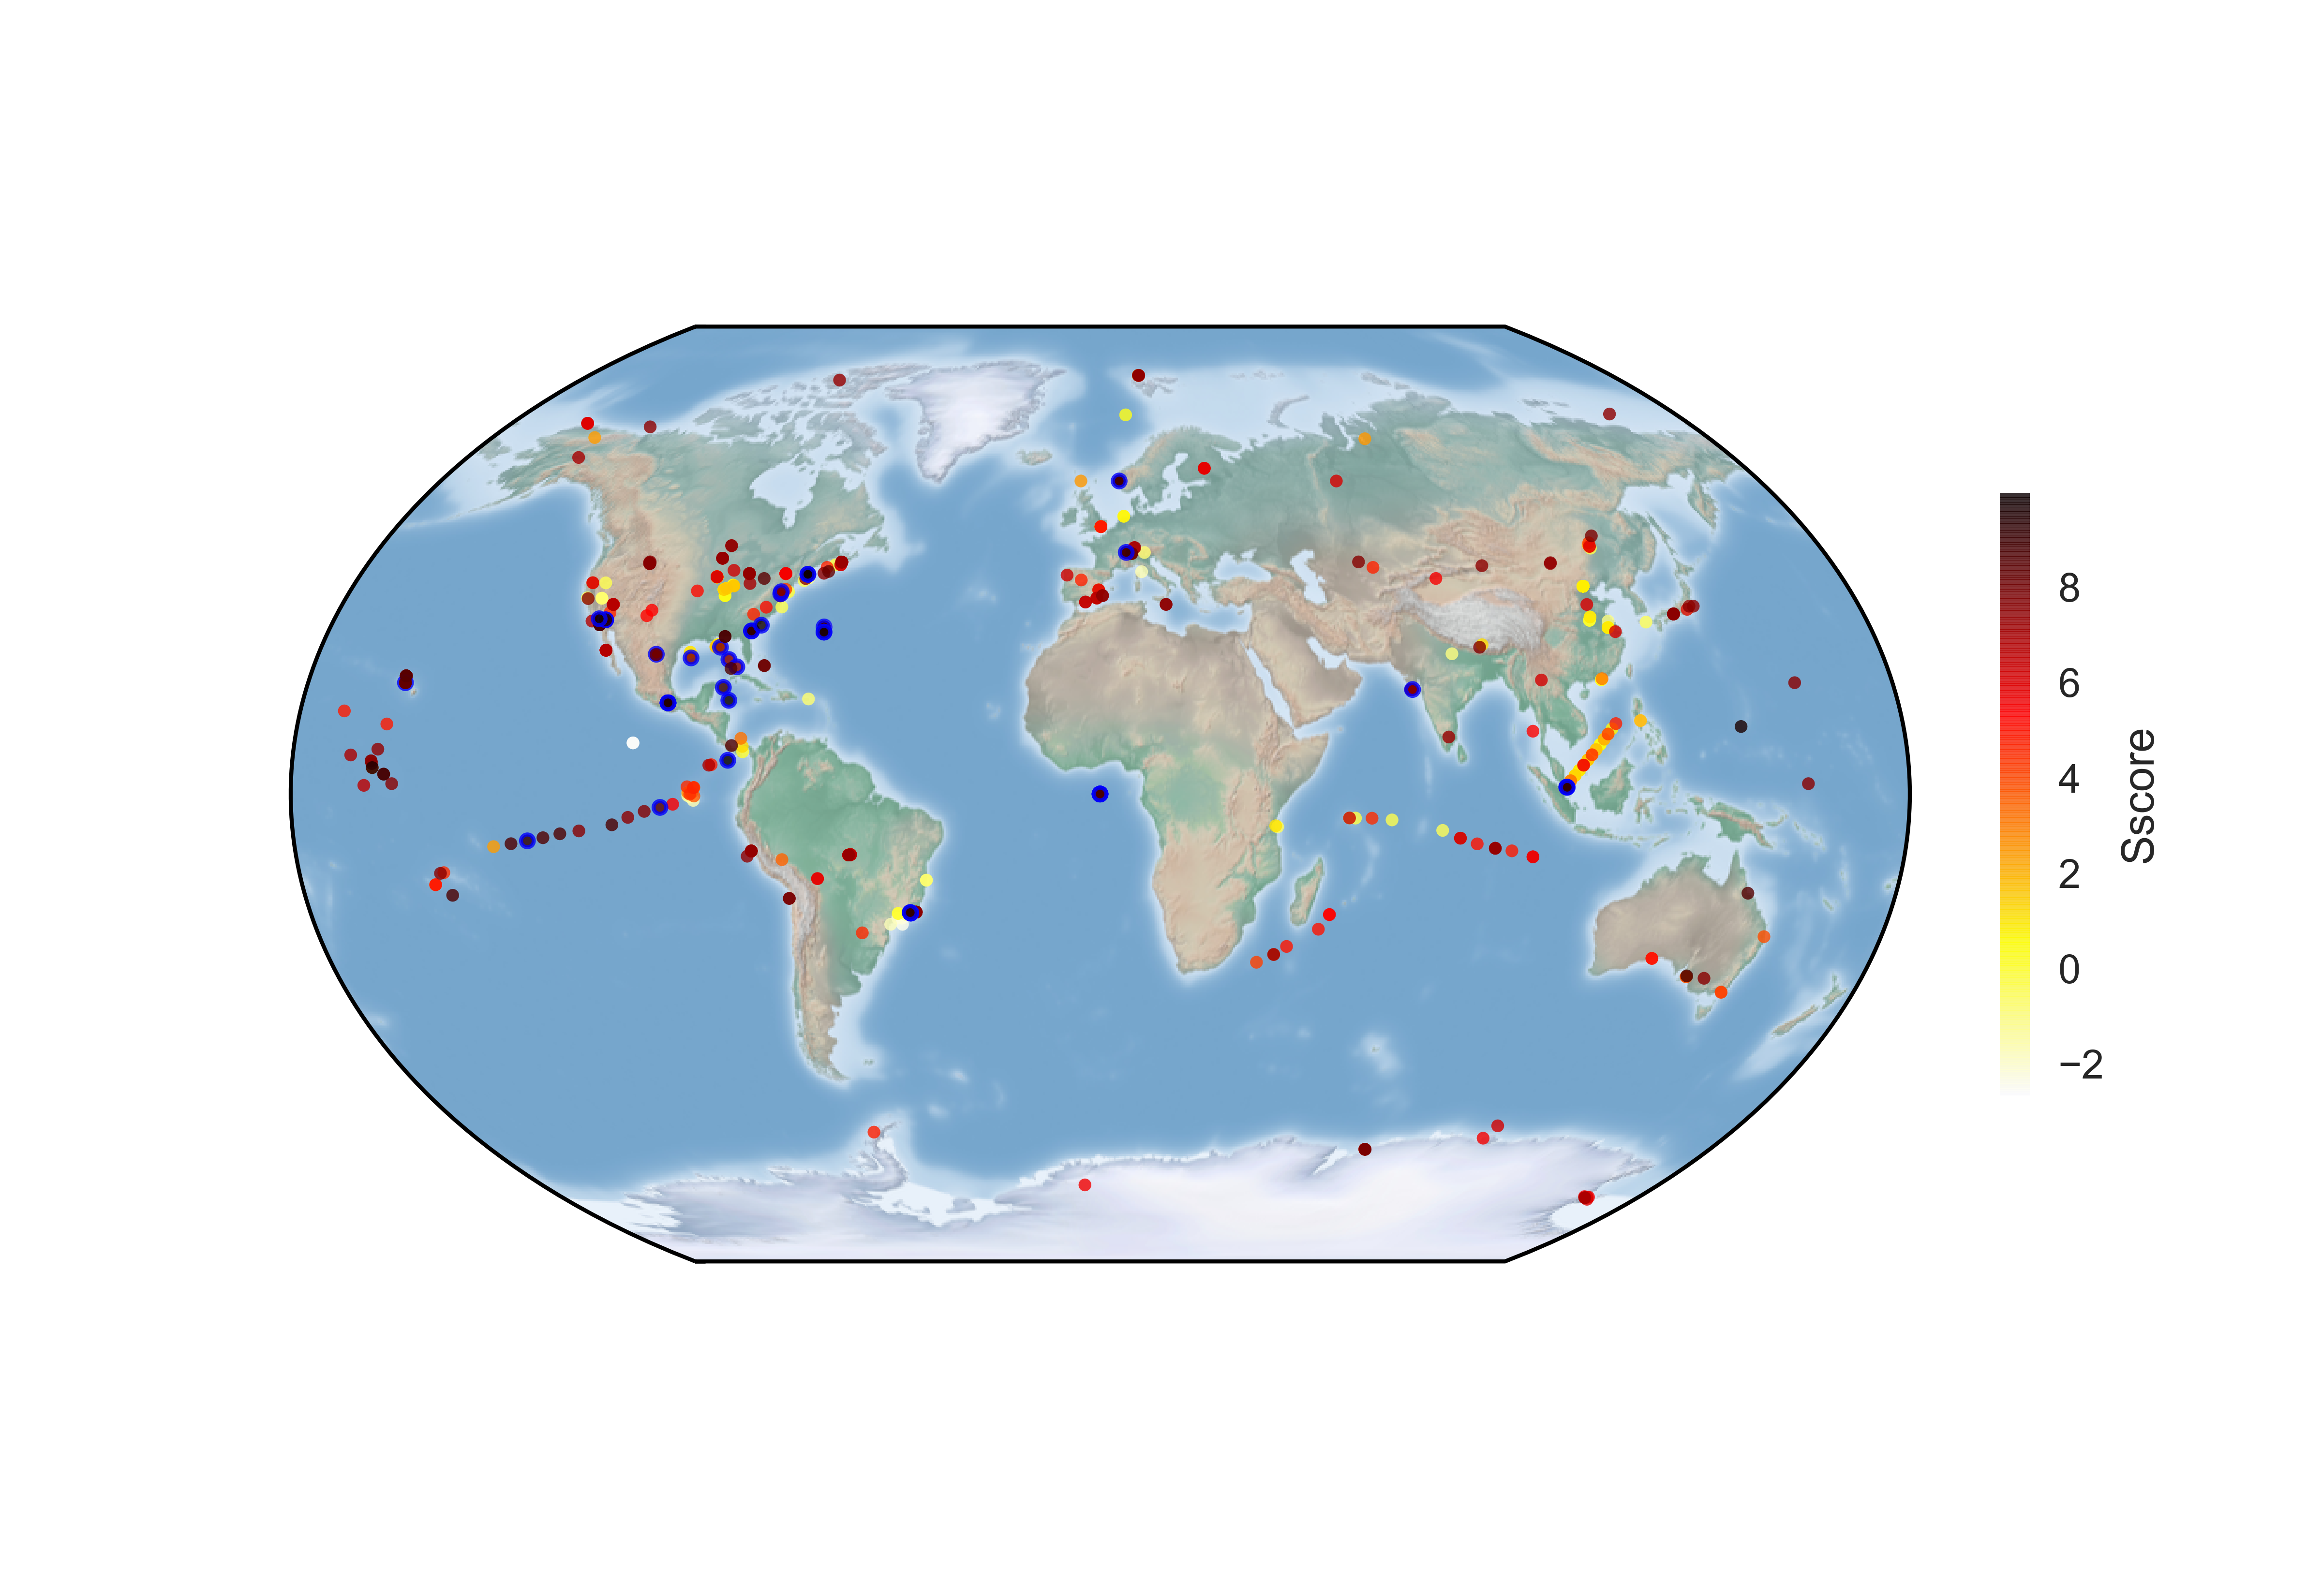
\includegraphics[width=160mm, scale =1]{world_map_SS.png}
    \caption{Distribution of the Sulfur Score in the metagenomes with geographical localization. The blue circles indicates Metagenomes above the 95 percentile}
        \label{fig:differential}
\end{figure}

\subsubsection{Computing the Score using different Pfams an plot KEGG map
abundancies}

The above mentioned options explain how to compute the Entropy Score using all
the Pfam's found in the input genes. In our case, from a database of 152 sulfur
protein-coding genes, we found 114 Pfam's which were used to compute the Score.

However, it is possible to choose specific Pfam's that are found in the input
genes. For example, from the 112 Pfam's we can choose a subset of 10 or 50
Pfam's that are know to be specific to certain routes or metabolic pathways.

In the case of Sulfur Cycle, we divided the metabolic pathways according to the
mayor reactions described \href{http://www.genome.jp/kegg/}{KEGG},
\href{https://metacyc.org/}{MetaCyc} and primary literature. The division of
the metabolic pathways of Sulfur Cycle is observed in Table
\ref{division_paths} 

Using the output derived from Interproscan (Stage \ref{stage2}) and
cross-reference using  \href{http://www.uniprot.org/}{UniProt}, we generated a
curated database of the genes involved in the Sulfur cycle (See file
/input\_data/sucy\_database.tab). Then, we divided each Pfam with their
corresponding molecular-level functions stored in  KO (KEGG Orthology). Due to
the domain composition of each protein, the same K0 may have several associated
Pfams and vise verse, one domain Pfam, could be present in several proteins or
KO's.  

Therefore, the Pfam entropy score \textit{entropy\_score.pl}  algorithm
(\ref{entropy_score}) is also able to compute the SS using specific Pfam's 
belonging to certain metabolic pathways. In order to use this option you  need
to enumerate the pathways of interest (arbitrarily) (As explained above  and
specify the Pfam's belonging to those pathways. See the,
/input\_data/sulfur\_score\_kegg\_list 

Besides is another option of SS that help you to visualize the 
Pfam's in the metabolic pathway of KEGG (map00920), you will need 
to provide a list with the Pfam id and the equivalent KO number 
(Note that Pfam's constitute partial domains of a protein, 
therefore, one Pfam, may be represented in several KO numbers). 
Example in  /input\_data/sulfur\_score\_kegg\_list

\begin{table}[H]
\centering
\caption{Metabolic pathways of global biogeochemical sulfur cycle divided by
numbers }
\label{division_paths}
\begin{tabular}{@{}lc@{}}
\toprule
Pathway                     & Number \\ \midrule
Sulfite oxidation           & 1      \\
Thiosulfate oxidation       & 2      \\
Tetrathionate oxidation     & 3      \\
Tetrathionate reduction     & 4      \\
Sulfate reduction DS        & 5      \\
S° reduction                & 6      \\
Thiosulfate disproportion   & 7      \\
Carbon disulfide oxidation  & 8      \\
Alkanesulfonate degradation & 9      \\
Sulfate reduction A         & 10     \\
Sulfide oxidation           & 11     \\
Cysteate oxidation          & 12     \\
Dimethylsulfone oxidation   & 13     \\
Sulfoacetate oxidation      & 14     \\
Sulfolactate oxidation      & 15     \\
DMS oxidation               & 16     \\
DMSP oxidation              & 17     \\
MTP oxidation               & 18     \\
Suloacetaldehyde oxidation  & 19     \\
S° oxidation                & 20     \\
S° disproportion            & 21     \\
Methanesulfonate oxidation  & 22     \\
Taurine oxidation           & 23     \\
DMS methanogenesis          & 24     \\
MTP methanogesis            & 25     \\
Methanethiol methanogenesis & 26     \\
SQDG biosynthesis           & 28     \\ \bottomrule
\end{tabular}
\end{table}

\begin{verbatim}
for msl in 30 60 100 150 200 250 300   
do      for path in {1..29}
do              for file in *.tab; do perl /home/valdeanda
/src/metagenome_Pfam_score-master/scripts/pfam_score.pl  pfam_score.pl 
-input $file  -size $msl -matrixdir /home/valdeanda
/src/metagenome_Pfam_score-master/data/entropies_matrix/ -pathway 
$path -keggmap /home/valdeanda/src/metagenome_Pfam_score-master
/input_data/sulfur_score_kegg_list  > $file.$msl.$path.score 
done
        done
                done
\end{verbatim}
\subsection{Random Score}

To compute score  using several percent of Pfams as input. 

\begin{verbatim}
#Locate all the metagenomes of the same MSL in a 
specific folder and the run the following script  


#!/bin/bash
for file  in *.tab
 do  for r  in {1..1000}
      do perl scripts/pfam_score.pl  pfam_score.pl -input  $file  -size 500
-matrixdir
/home/valdeanda/src/metagenome_Pfam_score-master/data/entropies_matrix/ -random
50  > random_test_50/$file.$r.score
        done
      done

#Obtain the random scores values using the following 
script: 

perl scripts/extract_random_scores.pl -dire <directory 
containing the random scores>
     


\end{verbatim}







\end{document}
